\documentclass[11pt]{article}
\usepackage[]{authblk}
\usepackage{graphicx}
\usepackage{tabularx}
%\usepackage{color}
\usepackage{colortbl}
\usepackage[usenames,dvipsnames,table]{xcolor}
\usepackage{booktabs}
\usepackage{longtable}
\usepackage{hanging}
\usepackage{indentfirst}
\usepackage{setspace}
\usepackage{enumitem}
\usepackage{verbatim}
\usepackage{upgreek}
\usepackage{framed}
\usepackage{ textcomp }
\usepackage{url}
\usepackage{soul}
\usepackage{amsmath, amsfonts,amssymb,mathrsfs}
\usepackage{fancyhdr}
\usepackage[compact]{titlesec}
\usepackage[T1]{fontenc}
\usepackage{lmodern}
\usepackage{float}

%\usepackage[backend=bibtex,hyperref=true,citestyle=authoryear,bibstyle=authortitle,firstinits=true,terseinits=true,doi=false,url=false,maxbibnames=10,maxcitenames=2]{biblatex}
%\addbibresource{../bib_tex/master_refs.bib}


\usepackage[sectionbib]{chapterbib}
\usepackage[sectionbib]{natbib}

%\DeclareCiteCommand{\cite}
  {\usebibmacro{prenote}}
  {\usebibmacro{citeindex}%
   \printtext[bibhyperref]{\usebibmacro{cite}}}
  {\multicitedelim}
  {\usebibmacro{postnote}}

\DeclareCiteCommand*{\cite}
  {\usebibmacro{prenote}}
  {\usebibmacro{citeindex}%
   \printtext[bibhyperref]{\usebibmacro{citeyear}}}
  {\multicitedelim}
  {\usebibmacro{postnote}}

\DeclareCiteCommand{\parencite}[\mkbibparens]
  {\usebibmacro{prenote}}
  {\usebibmacro{citeindex}%
    \printtext[bibhyperref]{\usebibmacro{cite}}}
  {\multicitedelim}
  {\usebibmacro{postnote}}

\DeclareCiteCommand*{\parencite}[\mkbibparens]
  {\usebibmacro{prenote}}
  {\usebibmacro{citeindex}%
    \printtext[bibhyperref]{\usebibmacro{citeyear}}}
  {\multicitedelim}
  {\usebibmacro{postnote}}

\DeclareCiteCommand{\footcite}[\mkbibfootnote]
  {\usebibmacro{prenote}}
  {\usebibmacro{citeindex}%
  \printtext[bibhyperref]{ \usebibmacro{cite}}}
  {\multicitedelim}
  {\usebibmacro{postnote}}

\DeclareCiteCommand{\footcitetext}[\mkbibfootnotetext]
  {\usebibmacro{prenote}}
  {\usebibmacro{citeindex}%
   \printtext[bibhyperref]{\usebibmacro{cite}}}
  {\multicitedelim}
  {\usebibmacro{postnote}}

\DeclareCiteCommand{\textcite}
  {\boolfalse{cbx:parens}}
  {\usebibmacro{citeindex}%
   \printtext[bibhyperref]{\usebibmacro{textcite}}}
  {\ifbool{cbx:parens}
     {\bibcloseparen\global\boolfalse{cbx:parens}}
     {}%
   \multicitedelim}
  {\usebibmacro{textcite:postnote}}

\newcommand{\citep}{\parencite}
\newcommand{\citet}{\textcite}
\defbibheading{relevref}[\refname]{\section*{Relevant References}}

\renewcommand{\postnotedelim}{\iffieldpages{postnote}{\addcolon}{\addcomma\space}} 
\DeclareFieldFormat{postnote}{#1} 

\DeclareFieldFormat[article, inbook, incollection, inproceedings, patent, thesis, unpublished]{title}{#1}
\DeclareFieldFormat[article, inbook, incollection, inproceedings, patent, thesis, unpublished]{journaltitle}{\mkbibemph{#1}\nopunct}
\DeclareFieldFormat[article, inbook, incollection, inproceedings, patent, thesis, unpublished]{volume}{{#1}\addcolon} %puts volume number in parens
%\DeclareFieldFormat[article, inbook, incollection, inproceedings, patent, thesis, unpublished]{year}{\mkbibparens{#1}\nopunct} %puts year in parens

\DeclareFieldFormat[article, incollection, patent, thesis, unpublished]{pages}{{\nopp#1}}

\DeclareFieldFormat{sentencecase}{\MakeSentenceCase{#1}}

\renewbibmacro*{title}{%
  \ifthenelse{\iffieldundef{title}\AND\iffieldundef{subtitle}}
    {}
    {\ifthenelse{\ifentrytype{article}\OR\ifentrytype{inbook}%
      \OR\ifentrytype{incollection}\OR\ifentrytype{inproceedings}%
      \OR\ifentrytype{inreference}}
      {\printtext[title]{%
        \printfield[sentencecase]{title}%
        \setunit{\subtitlepunct}%
        \printfield[sentencecase]{subtitle}}}%
      {\printtext[title]{%
        \printfield[titlecase]{title}%
        \setunit{\subtitlepunct}%
        \printfield[titlecase]{subtitle}}}%
     \newunit}%
  \printfield{titleaddon}}

\DefineBibliographyStrings{english}{% various adjustments to common bib entry strings
urlseen = {Accessed:},% What goes in front of the date a URL was accessed/retrieved etc.
editor = {(Ed)},%Ed – no dot, in brackets
editors = {(Eds)},% Eds – no dot, in brackets
byeditor = {(Ed.)}}% ‘Edited by’ for edited works

\DeclareNameAlias{default}{last-first}

\renewbibmacro{in:}{}

\renewbibmacro{publisher+location+date}{
  \iflistundef{publisher}
    {}
    {\printlist{publisher}%
       {\addcomma\space}%
      \iflistundef{location}
        {}
        {\printlist{location}}%
    }
}

\DeclareBibliographyDriver{article}{%
\usebibmacro{bibindex}%
\usebibmacro{begentry}%
\usebibmacro{author/translator+others}%
\newunit\newblock
\printfield{year}%
\setunit{\labelnamepunct}\newblock
\usebibmacro{title}%
\newunit
\printlist{language}%
\newunit\newblock
\usebibmacro{byauthor}%
\newunit\newblock
\usebibmacro{bytranslator+others}%
\newunit\newblock
\printfield{version}%
\newunit\newblock
%\usebibmacro{in:}% %mit in:
\usebibmacro{journal}%
\newunit\newblock
\printfield{volume}%
\newunit\newblock
\usebibmacro{byeditor+others}%
\newunit\newblock
\usebibmacro{note+pages}%
\newunit\newblock
\iftoggle{bbx:isbn}
{}%
\newunit\newblock
\usebibmacro{doi+eprint+url}%
\newunit\newblock
\usebibmacro{addendum+pubstate}%
\newunit\newblock
\usebibmacro{pageref}%
\usebibmacro{finentry}}

\DeclareBibliographyDriver{inproceedings}{%
\usebibmacro{bibindex}%
\usebibmacro{begentry}%
\usebibmacro{author/translator+others}%
\newunit\newblock
\printfield{year}%
\setunit{\labelnamepunct}\newblock
\usebibmacro{title}%
\newunit
\printlist{language}%
\newunit\newblock
\usebibmacro{byauthor}%
\newunit\newblock
\usebibmacro{bytranslator+others}%
\newunit\newblock
\printfield{version}%
\newunit\newblock
%\usebibmacro{in:}% %mit in:
\usebibmacro{booktitle}%
\newunit\newblock
\printfield{volume}%
\newunit\newblock
\usebibmacro{byeditor+others}%
\newunit\newblock
\usebibmacro{publisher+location+date}%
\newunit\newblock
\usebibmacro{note+pages}%
\newunit\newblock
\usebibmacro{pageref}%
\usebibmacro{finentry}}

\DeclareBibliographyDriver{book}{%
\usebibmacro{bibindex}%
\usebibmacro{begentry}%
\usebibmacro{author/translator+others}%
\newunit\newblock
\printfield{year}%
\setunit{\labelnamepunct}\newblock
\usebibmacro{title}%
\newunit
\printlist{language}%
\newunit\newblock
\usebibmacro{byauthor}%
\newunit\newblock
\usebibmacro{bytranslator+others}%
\newunit\newblock
%\usebibmacro{in:}% %mit in:
\usebibmacro{booktitle}%
\newunit\newblock
\printfield{volume}%
\newunit\newblock
\usebibmacro{publisher+location+date}%
\newunit\newblock
\usebibmacro{note+pages}%
\newunit\newblock
\usebibmacro{pageref}%
\usebibmacro{finentry}}





\setlength{\evensidemargin}{0in}
\setlength{\headheight}{0in}
\setlength{\headsep}{0in}
\setlength{\oddsidemargin}{-0.25in}
\setlength{\paperheight}{11in}
\setlength{\paperwidth}{8.5in}
\setlength{\tabcolsep}{0in}
\setlength{\textheight}{9in}
\setlength{\textwidth}{7in}
\setlength{\topmargin}{0in}
\setlength{\topskip}{0in}
\setlength{\voffset}{0in}
\parskip = 0.15in
\pagestyle{plain}
\setlength{\parindent}{0cm}

\definecolor{citescol}{RGB}{194,101,1}
\definecolor{urlscol}{RGB}{0,150,206}
\definecolor{linkscol}{RGB}{149,0,207}
\definecolor{mycol}{RGB}{25,23,191}
\definecolor{outputcol}{RGB}{34,139,34}
\definecolor{tcol}{RGB}{165,0,14}


\DeclareMathAlphabet{\msfsl}{T1}{cmr}{m}{it}
\DeclareMathAlphabet{\msyf}{OMX}{pcr}{m}{it}
\newcommand{\alf}{\upalpha}
\newcommand{\hilight}[1]{\colorbox{yellow}{#1}}

\newcommand{\levelone}[1]{
\bigskip
\noindent{\LARGE{\textsc{#1}}}
\vspace {0.05in}
}

\newcommand{\leveltwo}[1]{
\bigskip
\noindent{\Large{\textit{#1}}}
\vspace {-1mm}
}

\newcommand{\descriptionhead}[1]{
\noindent{\textbf{\textit{#1}}}\\ \vspace{-7mm}
}

\newcommand{\dhead}[1]{
\noindent{\textbf{\textit{#1 --}}}
}


\newcommand{\exs}[1]{
\vspace{-4mm}
\begin{itemize}
\item #1 \\ \vspace{-8mm}
\end{itemize}
}

\newcommand{\nbo}[1]{{\color{red}{#1}}}


\newcommand{\stepbullet}{\noindent \textbullet \ }
\newcommand{\mi}[1]{\textbf{\textit{#1}}}


\newcommand{\levelthree}[1]{\textit{#1 --}}


%\bibliographystyle{apalike}
%\bibpunct[; ]{(}{)}{;}{a}{,}{;}


\usepackage[breaklinks]{hyperref}
\usepackage[all]{hypcap}
\hypersetup{colorlinks=true,linkcolor=linkscol,citecolor=citescol,urlcolor=urlscol}


\newcommand{\R}{\texttt{R} }
\newcommand{\TESS}{\texttt{TESS}}
\newcommand{\PBD}{\texttt{PBD}}
\newcommand{\DDD}{\texttt{DDD}}
\newcommand{\Laser}{\texttt{laser}}
\newcommand{\TreePar}{\texttt{TreePar}}
\newcommand{\diversitree}{\texttt{diversitree}}
\newcommand{\RevBayes}{\texttt{RevBayes}}
\newcommand{\Rev}{\texttt{Rev}}
\newcommand{\MrBayes}{\texttt{MrBayes}}
\newcommand{\BEAST}{\texttt{BEAST}}
\newcommand{\PhyloBayes}{\texttt{PhyloBayes}}
\newcommand{\PAML}{\texttt{PAML}}
\newcommand{\Phylowood}{\texttt{Phylowood}}
\newcommand{\Tracer}{\texttt{Tracer}}


\let\otheriint\iint
\let\iint\relax
\usepackage{ wasysym }

\usepackage{framed}
\usepackage[]{listings}
%\usepackage{fontspec}
\usepackage{placeins}
\usepackage{epstopdf}

\lstset{breaklines=true}

\lstdefinestyle{textboxSmall}{
  language=Matlab,
  stepnumber=1,
  numbersep=10pt,
  tabsize=4,
  showspaces=false,
  showstringspaces=false
}

\definecolor{shadecolor}{RGB}{238,224,229}

\setlength{\tabcolsep}{5pt}
\setlength{\topmargin}{-0.4in}
\setlength{\headheight}{14.5pt}
\pagestyle{fancy}

\newcommand{\taha}[1]{{\textcolor{red}{[TAH comment: #1]}}} % TAH comment

\titlespacing{\section}{0pt}{*0}{*0}
\titlespacing{\subsection}{0pt}{*0}{*0}
\titlespacing{\subsubsection}{0pt}{*0}{*0}

\titleformat{\section}
  {\normalfont\Large\bfseries\color{mycol}}
  {\thesection}{1em}{}

\titleformat{\subsection}
  {\normalfont\large\bfseries\color{mycol}}
  {\thesubsection}{1em}{}

\titleformat{\subsubsection}
  {\normalfont\bfseries\color{mycol}}
  {\thesubsubsection}{1em}{}

% command for MrBayes command-line step
\newcommand{\cl}[1]{{\texttt{\textbf{#1}}}}

\newcommand{\colx}[1]{{\textcolor{tcol}{#1}}}

\newcommand{\rbprmt}{ > } 
\newcommand{\rbcl}[1]{\exs{\cl{\rbprmt{#1}}}}
\newcommand{\rbout}[1]{\cl{\textcolor{outputcol}{#1}}}
\newcommand{\rbdn}{{\Large \symbol{126}}} % This makes a copy/pasteable tilde
\newcommand{\rbclml}[1]{\exs{\cl{\ \ \ \ \ \ \ \ \ \ \ {#1}}}}

% Abbreviations
\newcommand{\IE}{i.e., }
\newcommand{\EG}{e.g., }
\newcommand{\CF}{cf. }
\newcommand{\IID}{i.i.d. }


% text box settings
% requires compiling w/ XeLaTeX
%\newfontfamily\listingsfont[Scale=1.0]{Courier New}
%\lstset{basicstyle=\listingsfont, columns=texcl}
%\defaultfontfeatures{Mapping=tex-text}

%\lstset{columns=fullflexible}
%\lstset{basicstyle=\ttfamily,columns=flexible}
\lstdefinelanguage{Rev}
{morekeywords={RevBayes},
sensitive=false,
morecomment=[l]{\#},
moredelim=[il][\color{gray}\ttfamily]{|*},
}
%\lstdefinelanguage{Rev}
%{morecomment=[l]{#},
%moredelim=[il][\color{gray}\ttfamily]{|*},
%}
\lstset{
    language=Rev,
    basicstyle=\ttfamily,
    columns=flexible
}
%\lstset{morecomment=[l]{\#}}


% Some commands to keep the sysbio.bst from generating weird errors
\newcommand{\bibAnnoteFile}[1]{%
\IfFileExists{#1}{\begin{quotation}\noindent\textsc{Key:} #1\\
\textsc{Annotation:}\ \input{#1}\end{quotation}}{}}

\newcommand{\bibAnnote}[2]{%
\begin{quotation}\noindent\textsc{Key:} #1\\
\textsc{Annotation:}\ #2\end{quotation}}

\bibliographystyle{sysbio}
\bibpunct[; ]{(}{)}{;}{a}{}{;}



\makeatletter
\lst@CCPutMacro\lst@ProcessOther {"2D}{\lst@ttfamily{-{}}{-{}}}
\@empty\z@\@empty
\makeatother

% commands
\newcommand{\impmark}{\strut\vadjust{\domark}}
\newcommand{\domark}{%
  \vbox to 0pt{
    \kern-\dp\strutbox
    \smash{\llap{$\rightarrow$\kern1em}}
    \vss
  }%
}


%\usepackage{paralist}
%\usepackage{algorithm}
%\usepackage{algpseudocode}
%\usepackage{enumitem}

\begin{document}
\renewcommand{\headrulewidth}{0.5pt}
\headsep = 20pt
\lhead{ }
\rhead{\textsc {\RevBayes~Tutorial --- State-Dependent Diversification Rate Estimation}}

\thispagestyle{plain}
\begin{center}

\textbf{\LARGE Phylogenetic Inference using \RevBayes}\\\vspace{2mm}
\textbf{\it{\Large State-Dependent Diversification Rate Estimation}}\\\vspace{2mm}
\vspace{1cm}
{\Large Sebastian H{\"o}hna, Will Freyman, and Emma Goldberg}
\vspace{1cm}
\end{center}

\def \ResourcePath {./}
\def \GlobalResourcePath {../}

\section*{Estimating Character State-Dependent Speciation \& Extinction Rates}

\subsection*{Introduction}

This tutorial describes how to specify character state-dependent branching process models in \RevBayes.
Frequently referred to as state-dependent speciation and extinction (SSE) models,
these models are a birth-death process where the diversification rates are dependent on the state of an evolving character.
The original model of this type considered a binary character (a trait with two discrete state values; called BiSSE, \citealt{Maddison2007}).
Several variants have also been developed for other types of traits \citep{FitzJohn2010, Goldberg2011, Goldberg2012, MagnusonFord2012, FitzJohn2012, Beaulieu2016, Freyman2017}.

We will outline the theory behind this method, and then you will fit it to data using Markov chain Monte Carlo (MCMC).
\RevBayes is a powerful tool for SSE analyses. After working through this tutorial you
should be able to set up custom SSE models and use them to
infer character-dependent diversification rates, ancestral states, and stochastic character maps.
We also provide examples of how to plot the results using the \RevGadgets R package.

\subsection*{Contents}

The State-Dependent Speciation and Extinction tutorial contains several sections:

\begin{itemize}
\item Section \ref{sec:diversification_rate_overview}: Introduction to diversification rate estimation
\item Section \ref{sec:models}: Theory behind diversification rate models
\item Section \ref{sec:BiSSE_Theory}: Theory behind SSE models
\item Section \ref{sec:CDBDP}: Running a BiSSE/MuSSE analysis in \RevBayes
\item Section \ref{sec:HiSSE_Theory}: Running a HiSSE analysis in \RevBayes
\item Section \ref{sec:ClaSSE}: Running a ClaSSE analysis in \RevBayes
\end{itemize}

\subsection*{Requirements}

We assume that you have read and hopefully completed the following tutorials:
\begin{itemize}
\item \href{https://github.com/revbayes/revbayes_tutorial/raw/master/tutorial_TeX/RB_Getting_Started/RB_Getting_Started.pdf}{Getting started}
\item \href{https://github.com/revbayes/revbayes_tutorial/raw/master/tutorial_TeX/RB_Basics_Tutorial/RB_Basics_Tutorial.pdf}{\Rev basics}
\item \href{https://github.com/revbayes/revbayes_tutorial/raw/master/tutorial_TeX/RB_DiversificationRate_Tutorial/RB_DiversificationRate_Tutorial.pdf}{Basic Diversification Rate Estimation}
\end{itemize}
Note that the \href{https://github.com/revbayes/revbayes_tutorial/raw/master/tutorial_TeX/RB_Basics_Tutorial/RB_Basics_Tutorial.pdf}{\Rev basics tutorial} introduces the basic syntax of \Rev but does not cover any phylogenetic models.
You may skip the \href{https://github.com/revbayes/revbayes_tutorial/raw/master/tutorial_TeX/RB_Basics_Tutorial/RB_Basics_Tutorial.pdf}{\Rev basics tutorial} if you have some familiarity with \R.
We tried to keep this tutorial very basic and introduce all the language concepts and theory on the way.
You may only need the \href{https://github.com/revbayes/revbayes_tutorial/raw/master/tutorial_TeX/RB_Basics_Tutorial/RB_Basics_Tutorial.pdf}{\Rev basics tutorial} for a more in-depth discussion of concepts in \Rev.

%%%%%%%%%%%%%%
%%   DATA   %%
%%%%%%%%%%%%%%
\section*{Data and files} \label{sec:data_files}

We provide the data files which we will use in this tutorial.
You may want to use your own data instead.
In the \cl{data} folder, you will find the following files:
\begin{itemize}

    \item \href{https://github.com/revbayes/revbayes_tutorial/raw/master/RB_DiversificationRate_CharacterDependent_Tutorial/data/primates_tree.nex}{primates\_tree.nex}:
        Dated primate phylogeny including 233 out of 367 species.
        (This tree is from \citealt{MagnusonFord2012}, who took it from \citealt{Vos2006} and then randomly resolved the polytomies using the method of \citealt{Kuhn2011}.)

    % Not actually used in this tutorial.
    % \item \href{https://github.com/revbayes/revbayes_tutorial/raw/master/RB_DiversificationRate_CharacterDependent_Tutorial/data/primates_habitat.nex}{primates\_habitat.nex}:
    %     Habitat data (also from \citealt{MagnusonFord2012}).

    \item \href{https://github.com/revbayes/revbayes_tutorial/raw/master/RB_DiversificationRate_CharacterDependent_Tutorial/data/primates_morph.nex}{primates\_morph.nex}:
        A set of several discrete-valued characters. % from where?
        The characters are described in the file \href{https://github.com/revbayes/revbayes_tutorial/raw/master/RB_DiversificationRate_CharacterDependent_Tutorial/data/primates_morph_description.txt}{primates\_morph\_description.txt}.

    \item \href{https://github.com/revbayes/revbayes_tutorial/raw/master/RB_DiversificationRate_CharacterDependent_Tutorial/data/primates_biogeo.tre}{primates\_biogeo.tre}: 
        A dated phylogeny of the 23 primate species. % from M. Landis' biogeo DEC tutorial, not sure where he got it from...
    
    \item \href{https://github.com/revbayes/revbayes_tutorial/raw/master/RB_DiversificationRate_CharacterDependent_Tutorial/data/primates_biogeo.tsv}{primates\_biogeo.tsv}:
        Biogeographic range data for 23 primate species.

\end{itemize}

\impmark{Open the tree files \cl{primates\_tree.nex} and \cl{primates\_biogeo.tre} in FigTree.}

\impmark{Open the character data files \cl{primates\_morph.nex} and \cl{primates\_biogeo.tsv} in a text editor.}

\newpage


\section{Overview: Diversification Rate Estimation}

Models of speciation and extinction are fundamental to any phylogenetic analysis of macroevolutionary processes.
A prior describing the distribution of speciation events over time is critical to estimating phylogenies with branch lengths proportional to time.
Moreover, stochastic branching models allow for inference of speciation and extinction rates.
These inferences allow us to investigate key questions in evolutionary biology.

Similarly, diversification-rate parameters are also included as nuisance parameters of other phylogenetic models---\IE where these diversification-rate parameters are not of direct interest.
For example, many methods for estimating species divergence times---such as \BEAST \citep{Drummond2012}, \MrBayes \citep{Ronquist2012}, and \RevBayes \citep{Hoehna2015}---implement `relaxed-clock models' that include a constant-rate birth-death branching process as a prior model on the distribution of tree topologies and node ages.
Although the parameters of these `tree priors' are not typically of direct interest, they are nevertheless estimated as part of the joint posterior probability distribution of the relaxed-clock model, and so can be estimated simply by querying the corresponding marginal posterior probability densities.
In fact, this may provide more robust estimates of the diversification-rate parameters, as they accommodate uncertainty in the other phylogenetic-model parameters (including the tree topology, divergence-time estimates, and the other relaxed-clock model parameters).

\subsection{Types of Hypotheses for Estimating Diversification Rates}


Many evolutionary phenomena entail differential rates of diversification (speciation -- extinction); \EG adaptive radiation, diversity-dependent diversification, key innovations, and mass extinction.
The specific study questions regarding lineage diversification may be classified within three fundamental categories of inference problems.
Admittedly, this classification scheme is somewhat arbitrary, but it is nevertheless useful, as it allows users to navigate the ever-increasing number of available phylogenetic methods.
Below, we describe each of the fundamental questions regarding diversification rates.

\paragraph{(1) Diversification-rate through time estimation}\textit{What is the (constant) rate of diversification in my study group?} 
The most basic models estimate parameters of the stochastic-branching process (\IE rates of speciation and extinction, or composite parameters such as net-diversification and relative-extinction rates) under the assumption that rates have remained constant across lineages and through time; \IE under a constant-rate birth-death stochastic-branching process model.
Extensions to the (basic) constant-rate models include diversification-rate variation through time.
First, we might ask whether there is evidence of an episodic, tree-wide increase in diversification rates (associated with a sudden increase in speciation rate and/or decrease in extinction rate), as might occur during an episode of adaptive radiation.
A second question asks whether there is evidence of a continuous/gradual decrease in diversification rates through time (associated with decreasing speciation rates and/or increasing extinction rates), as might occur because of diversity-dependent diversification (\IE where competitive ecological interactions among the species of a growing tree decrease the opportunities for speciation and/or increase the probability of extinction).
A final question in this category asks whether our study tree was impacted by a mass-extinction event (where a large fraction of the standing species diversity is suddenly lost).



\paragraph{(2) Diversification-rate variation across branches estimation}\textit{Is there evidence that diversification rates have varied significantly across the branches of my study group?}
Models have been developed to detect departures from rate constancy across lineages; these tests are analogous to methods that test for departures from a molecular clock---\IE to assess whether substitution rates vary significantly across lineages.
These models are important for assessing whether a given tree violates the assumptions of other inference methods.
Furthermore, these models are important to answer questions such as:
\textit{What are the branch-specific diversification rates?}; and
\textit{Have there been significant diversification-rate shifts along branches in my study group, and if so, how many shifts and along which branches?}


\paragraph{(3) Character-dependent diversification-rate estimation}\textit{Are diversification rates correlated with some variable in my study group?}
Character-dependent diversification-rate models aim to identify overall correlations between diversification rates and organismal features (binary and multi-state discrete morphological traits, continuous morphological traits, geographic range, etc.).
For example, one can hypothesize that a binary character, say if an organism is herbivorous/carnivorous or self-compatible/self-incompatible, impact the diversification rates.
Then, if the organism is in state 0 (\EG is herbivorous) it has a lower (or higher) diversification rate than if the organism is in state 1 (\EG carnivorous).


%Questions regarding mass-extinction events can be inferred using \TESS by performing specific hypothesis tests (see Section~\ref{sec:mass-extinction}) or analyses under the CPP on Mass-Extinction Times (\CoMET) model \citep{May2015}.
%These analyses can identify whether your study tree has been impacted by mass extinction, and if so, can identify the number and timing of these events.
%Additionally, the \CoMET model can be used to explore events other than mass extinction---such as the number of tree-wide diversification-rate shifts, the timing of those events, and the rate parameters (\EG speciation and extinction rates) associated with those events.
%However, the reliability to detect tree-wide diversification-rate shifts is currently being explored.
%We describe how to use \TESS and \CoMET to explore mass-extinction events in Section \ref{sec:CoMET} of this guide.


\section{Models}\label{sec:Models}

We begin this section with a general introduction to the stochastic birth-death branching process that underlies inference of diversification rates in \RevBayes.
This primer will provide some details on the relevant theory of stochastic-branching process models.
We appreciate that some readers may want to skip this somewhat technical primer; however, we believe that a better understanding of the relevant theory provides a foundation for performing better inferences.
We then discuss a variety of specific birth-death models, but emphasize that these examples represent only a tiny fraction of the possible diversification-rate models that can be specified in \RevBayes.

\subsection{The birth-death branching process}
Our approach is based on the \textit{reconstructed evolutionary process} described by \cite{Nee1994b}; a birth-death process in which only sampled, extant lineages are observed.
Let $N(t)$ denote the number of species at time $t$.
Assume the process starts at time $t_1$ (the `crown' age of the most recent common ancestor of the study group, $t_\text{MRCA}$) when there are two species.
Thus, the process is initiated with two species, $N(t_1) = 2$.
We condition the process on sampling at least one descendant from each of these initial two lineages; otherwise $t_1$ would not correspond to the $t_\text{MRCA}$ of our study group.
Each lineage evolves independently of all other lineages, giving rise to exactly one new lineage with rate $b(t)$ and losing one existing lineage with rate $d(t)$ (Figure~\ref{fig:BirthDeathShift} and Figure~\ref{fig:BDP}).
Note that although each lineage evolves independently, all lineages share both a common (tree-wide) speciation rate $b(t)$ and a common extinction rate $d(t)$ \citep{Nee1994b,Hoehna2015a}.
Additionally, at certain times, $t_{\mathbb{M}}$, a mass-extinction event occurs and each species existing at that time has the same probability, $\rho$, of survival.
Finally, all extinct lineages are pruned and only the reconstructed tree remains (Figure \ref{fig:BirthDeathShift}).

\begin{figure}[h]
\centering
       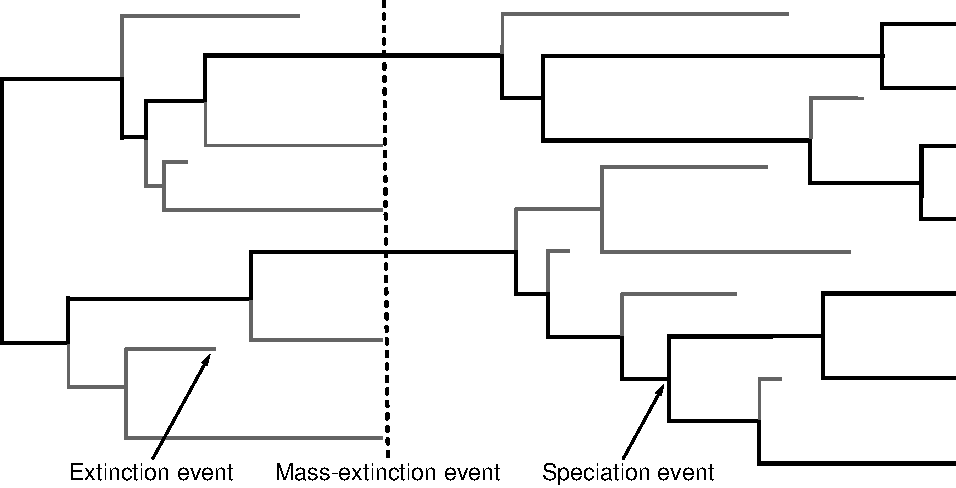
\includegraphics[width=0.8\textwidth]{\ResourcePath figures/BirthDeathShift.pdf}
   \caption{A realization of the  birth-death process with mass extinction.
   Lineages that have no extant or sampled descendant are shown in gray and surviving lineages are shown in a thicker black line.}
\label{fig:BirthDeathShift}
\end{figure}

\begin{figure}[!htbp]
  	\begin{center}
  		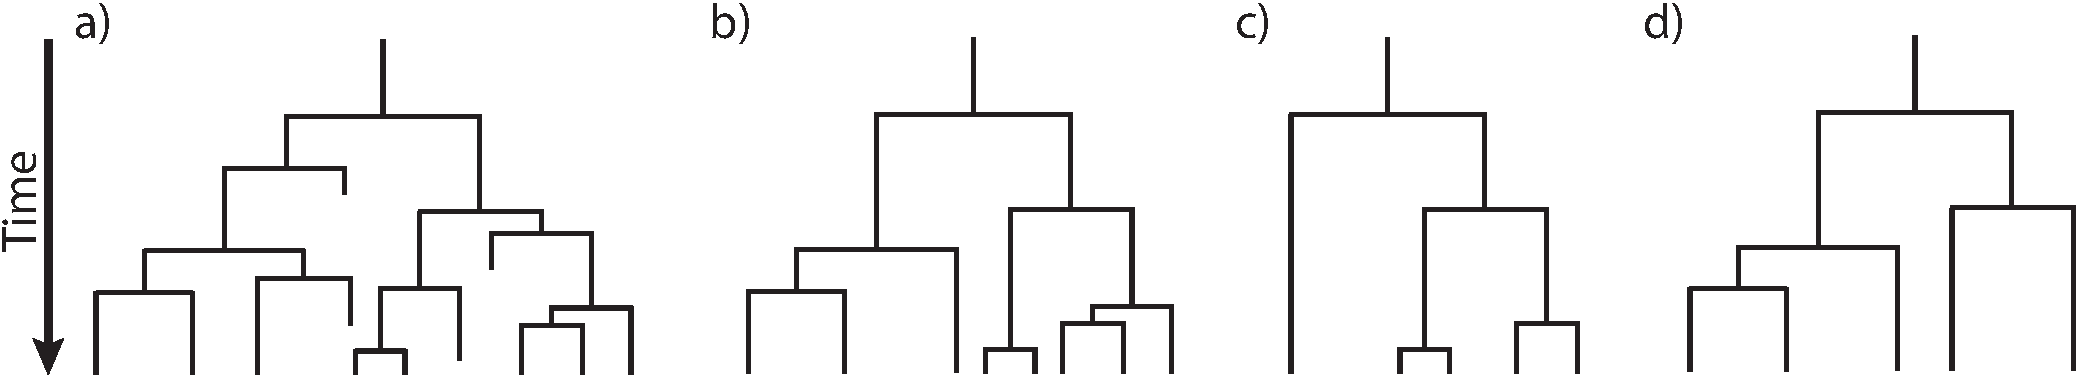
\includegraphics[width=\textwidth]{\ResourcePath figures/birth-death-sketch.pdf}
		\caption{
		{\bf Examples of trees produced under a birth-death process.}
		The process is initiated at the first speciation event (the `crown-age' of the MRCA) when there are two initial lineages.
		At each speciation event the ancestral lineage is replaced by two descendant lineages.
		At an extinction event one lineage simply terminates.
		(A) A complete tree including extinct lineages.
		(B) The reconstructed tree of tree from A with extinct lineages pruned away.
		(C) A \emph{uniform} subsample of the tree from B, where each species was sampled with equal probability, $\rho$.
		(D) A \emph{diversified} subsample of the tree from B, where the species were selected so as to maximize diversity.}
	\label{fig:BDP}
  	\end{center}
\end{figure}

To condition the probability of observing the branching times on the survival of both lineages that descend from the root, we divide by $P(N(T) > 0 | N(0) = 1)^2$.
Then, the probability density of the branching times, $\mathbb{T}$, becomes
\begin{align*}
P(\mathbb{T}) = \frac{\overbrace{P(N(T) = 1 \mid N(0) = 1)^2}^{\text{both initial lineages have one descendant}}}{ \underbrace{P(N(T) > 0 \mid N(0) = 1)^2}_{\text{both initial lineages survive}} } \times \prod_{i=2}^{n-1} \overbrace{i \times b(t_i)}^{\text{speciation rate}} \times \overbrace{P(N(T) = 1 \mid N(t_i) = 1)}^\text{lineage has one descendant},
\end{align*}
and the probability density of the reconstructed tree (topology and branching times) is then
\begin{align}
P(\Psi) = \; & \frac{2^{n-1}}{n!(n-1)!} \times \left( \frac{P(N(T) = 1 \mid N(0) = 1)}{P(N(T) > 0 \mid N(0) = 1)} \right)^2 \nonumber\\
		  \; & \times \prod_{i=2}^{n-1} i \times b(t_i) \times P(N(T) = 1 \mid N(t_i) = 1)
	\label{eq:tree_probability}
\end{align}

We can expand Equation~(\ref{eq:tree_probability}) by substituting $P(N(T) > 0 \mid N(t) =1)^2 \exp(r(t,T))$ for $P(N(T) = 1 \mid N(t) = 1)$, where $r(u,v) = \int^v_u d(t)-b(t)dt$; the above equation becomes
\begin{align}
P(\Psi) = \; & \frac{2^{n-1}}{n!(n-1)!} \times \left( \frac{P(N(T) > 0 \mid N(0) =1 )^2 \exp(r(0,T))}{P(N(T) > 0 \mid N(0) = 1)} \right)^2 \nonumber\\
		  \; & \times \prod_{i=2}^{n-1} i \times b(t_i) \times P(N(T) > 0 \mid N(t_i) = 1)^2 \exp(r(t_i,T)) \nonumber\\
		= \; & \frac{2^{n-1}}{n!} \times \Big(P(N(T) > 0 \mid N(0) =1 ) \exp(r(0,T))\Big)^2 \nonumber\\
		  \; & \times \prod_{i=2}^{n-1} b(t_i) \times P(N(T) > 0 \mid N(t_i) = 1)^2 \exp(r(t_i,T)).
		\label{eq:tree_probability_substitution}
\end{align}
For a detailed description of this substitution, see \cite{Hoehna2015a}.
Additional information regarding the underlying birth-death process can be found in \cite[Equation 3.4.6]{Thompson1975} and \cite{Nee1994b} for constant rates and \cite{Lambert2010,Lambert2013,Hoehna2013,Hoehna2014a,Hoehna2015a} for arbitrary rate functions.

To compute the equation above we need to know the rate function, $r(t,s) = \int_t^s d(x)-b(x) dx$, and the probability of survival, $P(N(T)\!>\!0|N(t)\!=\!1)$.
\cite{Yule1925} and later \cite{Kendall1948} derived the probability that a process survives ($N(T) > 0$) and the probability of obtaining exactly $n$ species at time $T$ ($N(T) = n$) when the process started at time $t$ with one species.
Kendall's results were summarized in Equation (3) and Equation (24) in \cite{Nee1994b}
\begin{eqnarray}
P(N(T)\!>\!0|N(t)\!=\!1) & = & \left(1+\int\limits_t^{T} \bigg(\mu(s) \exp(r(t,s))\bigg) ds\right)^{-1} \label{eq:survival} \\ \nonumber \\
P(N(T)\!=\!n|N(t)\!=\!1) & = & (1-P(N(T)\!>\!0|N(t)\!=\!1)\exp(r(t,T)))^{n-1} \nonumber\\
& & \times P(N(T)\!>\!0|N(t)\!=\!1)^2 \exp(r(t,T)) \label{eq:N} %\\
%P(N(T)\!=\!1|N(t)\!=\!1) & = & P(N(T)\!>\!0|N(t)\!=\!1)^2 \exp(r(t,T)) \label{eq:1}
\end{eqnarray}
An overview for different diversification models is given in \cite{Hoehna2015a}.





% Maybe the "Models" section isn't necessary?
%%%%%%%%%%%%%%%%%%%%
%%%    THEORY    %%%
%%%%%%%%%%%%%%%%%%%%
\section{Theory behind state-dependent diversification models} \label{sec:BiSSE_Theory}

The Binary State Speciation and Extinction model (BiSSE; \citealt{Maddison2007}) was introduced because of two problems identified by \citet{Maddison2006b}.
First, inferences about character state transitions based on simple transition models \citep[like][]{Pagel1999} can be thrown off if the character affects rates of speciation or extinction.
Second, inferences about whether a character affects lineage diversification based on sister clade comparisons \citep{Mitter1988} can be thrown off if the transition rates are asymmetric.
BiSSE and related models are now mostly used to assess if the states of a character are associated with different rates of speciation or extinction.

\RevBayes implements the extension of BiSSE to any number of discrete states (i.e., the MuSSE model in \diversitree; \citealt{FitzJohn2012}).
We will first describe the general theory about the model;
you may skip over this section if you are not interested in the math behind the model.
Then we will show how to run an analysis in \RevBayes.

\begin{figure}[h!]
\centering
\fbox{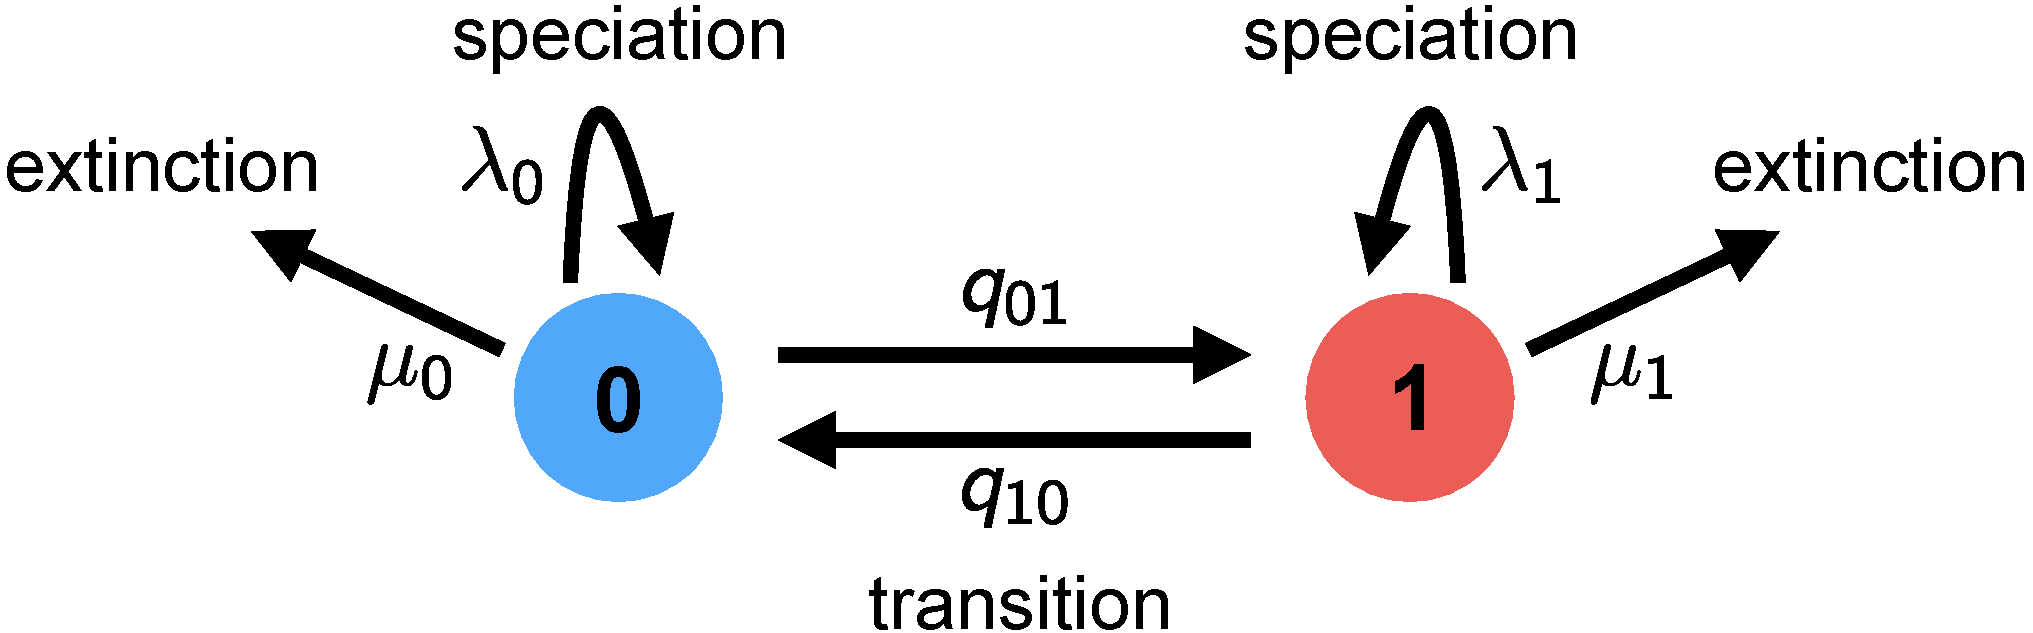
\includegraphics[width=0.7\textwidth]{\ResourcePath figures/BiSSE.pdf}}
\caption{\small
    A schematic overview of the \BiSSE model.
    Each lineage has a binary trait associated with it, so it is either in state 0 (blue) or state 1 (red).
    When a lineage is in state 0, it can either (a) speciate with rate $\lambda_0$ which results into two descendant lineage both being in state 0; (b) go extinct with rate $\mu_0$; or (c) transition to state 1 with rate $q_{01}$.
    The same types of events are possible when a lineage is in state 1 but with rates $\lambda_1$, $\mu_1$, and $q_{10}$, respectively.
}
\label{fig:BiSSE_Schematic}
\end{figure}

\subsection{General approach}

The \BiSSE model assumes two discrete states (\IE a binary character), and that the state of each extant species is known (\IE the discrete-valued character is observed).
The general approach adopted by \BiSSE and related models is to derive a set of ordinary differential equations (ODEs) that describe how the probability of observing a descendant clade changes along a branch in the observed phylogeny.
Each equation in this set describes how the probability of observing a clade changes through time if it is in a particular state over that time period; collectively, these equations are called $\frac{ \mathrm{d}D_{N,i}(t)}{\mathrm{d}t}$, where $i$ is the state of a lineage at time $t$ and $N$ is the clade descended from that lineage.

Computing the likelihood proceeds by establishing an initial value problem.
We initialize the procedure by observing the character states of some lineages, generally the tip states.
Then starting from those probabilities (\EG species X has state 0 with probability 1 at the present), we describe how those probabilities change over time (described by the ODEs), working our way back until we have computed the probabilities of observing that collection of lineages at some earlier time (\EG the root).

As we integrate from the tips to the root, we need to deal with branches coming together at nodes.
Assuming that the parent and daughter lineages have the same state, we multiply together the probabilities that the daughters are state $i$ and the instantaneous speciation rate $\lambda_i$ to get the initial value for the ancestral branch subtending that node.

Proceeding in this way down the tree results in a set of $k$ probabilities at the root; these $k$ probabilities represent the probability of observing the phylogeny conditional on the root being in each of the states (\IE the $i^\text{th}$ conditional probability is the probability of observing the tree given that the root is in state $i$).
The overall likelihood of the tree is a weighted average of the $k$ probabilities at the root, where the weighting scheme represents the assumed probability that the root was in each of the $k$ states.

As with all birth-death process models, special care must be taken to account for the possibility of extinction.
Specifically, the above ODEs must accommodate lineages that may arise along each branch in the tree that subsequently go extinct before the present (and so are unobserved).
This requires a second set of $k$ ODEs, $\frac{ \mathrm{d}E_{i}(t)}{\mathrm{d}t}$, which define how the probability of eventual extinction from state $i$ changes over time.
These ODEs must be solved to compute the differential equations $\frac{ \mathrm{d}D_{N,i}(t)}{\mathrm{d}t}$.
We will derive both sets of equations in the following sections.

% This framework therefore requires four distinct pieces of information to compute the likelihood of the data:
%	\begin{enumerate}
%		\item A set of ordinary differential equations describing how the probability of the data (observed lineages) changes through time, $\frac{ \mathrm{d}D_{N,i}(t)}{\mathrm{d}t}$.
%		\item A set of ordinary differential equations describing how the extinction probability of unobserved (extinct or unsampled) lineages changes through time, $\frac{ \mathrm{d}E_{i}(t)}{\mathrm{d}t}$.
%		\item An appropriate set of initial conditions.
%		\item An appropriate weighting scheme for the root probabilities.
%	\end{enumerate}

% In the following sections we detail how each of these components is determined for increasingly complex birth-death process models.

%%%%%%%%%%%%%%%%%%%%
%%%  BiSSE math  %%%
%%%%%%%%%%%%%%%%%%%%
\subsection{Derivation for the binary state birth-death process}

The derivation here follows the original description in \citet{Maddison2007}.
Consider a (time-independent) birth-death process with two possible states (a binary character), with diversification rates $\{\lambda_0, \mu_0\}$ and $\{\lambda_1, \mu_1\}$.

\subsubsection{Clade probabilities, $D_{N, i}$}
%%% D_i %%%

We define $D_{N,0}(t)$ as the probability of observing lineage $N$ descending from a particular branch at time $t$, given that the lineage at that time is in state 0.
To compute the probability of observing the lineage at some earlier time point, $D_{N,0}(t + \Delta t)$, we enumerate all possible events that could occur within the interval $\Delta t$.
Assuming that $\Delta t$ is small---so that the probability of more than one event occurring in the interval is negligible---there are four possible scenarios within the time interval (Fig.~\ref{fig:BiSSE_Events_D}):
\begin{enumerate}
	\item nothing happens;
	\item a transition occurs, so the state changes $0 \rightarrow 1$;
	\item a speciation event occurs, and the right descendant subsequently goes extinct before the present, or;
	\item a speciation event occurs and the left descendant subsequently goes extinct before the present.
\end{enumerate}
We are describing events within a branch of the tree (not at a node), so for (3) and (4), we require that one of the descendant lineages go extinct before the present because we do not observe a node in the tree between $t$ and $t + \Delta t$.

\begin{figure}
\centering
\fbox{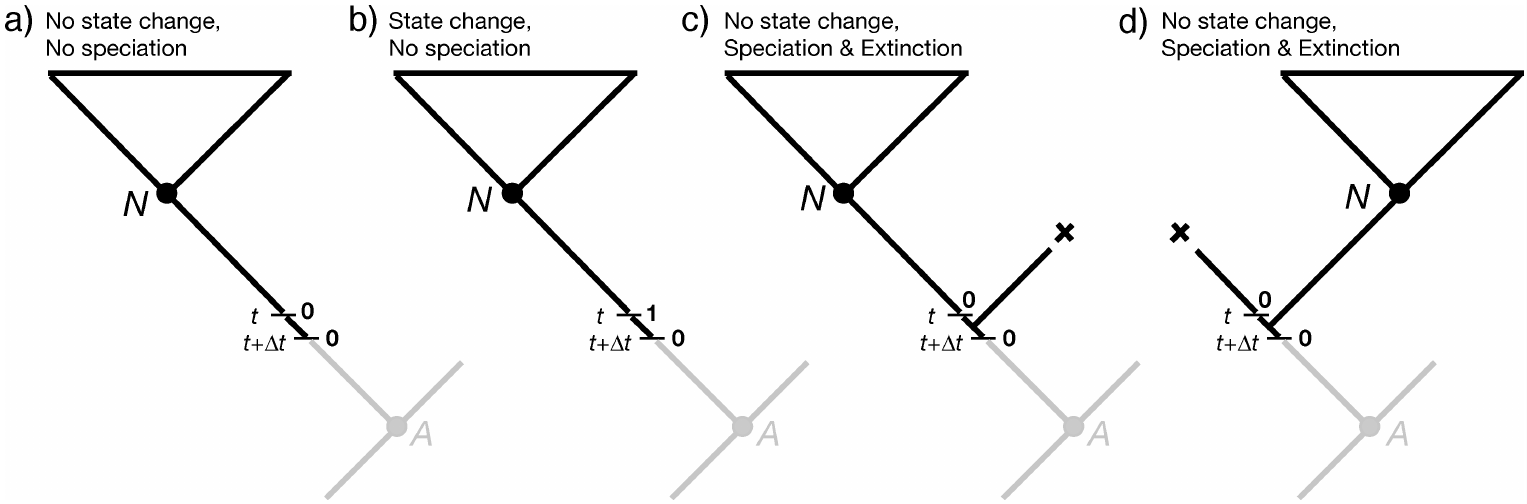
\includegraphics[width=\textwidth]{\ResourcePath figures/BiSSE_Events_D.png}}
\caption{\small
    Possible events along a branch in the BiSSE model, used for deriving $D_{N,0}(t + \Delta t)$.
    This is Figure 2 in \citet{Maddison2007}.
}
\label{fig:BiSSE_Events_D}
\end{figure}

We can thus compute $D_{N,0}(t + \Delta t)$ as:
\begin{align*}
	D_{N,0}(t + \Delta t) = & \;(1 - \mu_0 \Delta t) \times & \text{in all cases, no extinction of the observed lineage} \\
                         & \;[  (1 - q_{01} \Delta t)(1 - \lambda_0 \Delta t) D_{N,0}(t) & \text{case (1) nothing happens} \\
                         & \; + (q_{01} \Delta t) (1 - \lambda_0 \Delta t) D_{N,1}(t) & \text{case (2) state change but no speciation} \\
                         & \; + (1 - q_{01} \Delta t) (\lambda_0 \Delta t) E_0(t) D_{N,0}(t) & \text{case (3) no state change, speciation, extinction} \\
                         & \; + (1 - q_{01} \Delta t) (\lambda_0 \Delta t) E_0(t) D_{N,0}(t)] & \text{case (4) no state change, speciation, extinction}
\end{align*}
A matching equation can be written down for $D_{N,1}(t+\Delta t)$.

To convert these difference equations into differential equations, we take the limit $\Delta t \rightarrow 0$.
With the notation that $i$ can be either state 0 or state 1, and $j$ is the other state, this yields:
\begin{equation}
    \frac{\mathrm{d}D_{N,i}(t)}{\mathrm{d}t} = - \left(\lambda_i + \mu_i + q_{ij} \right) D_{N,i}(t) + q_{ij} D_{N,j}(t) + 2 \lambda_i E_i(t) D_{N,i}(t)
    \label{eq:BiSSE_D}
\end{equation}

\subsubsection{Extinction probabilities, $E_i$}
%%% E_i %%%

To solve the above equations for $D_{N, i}$, we see that we need the extinction probabilities.
Define $E_0(t)$ as the probability that a lineage in state 0 at time $t$ goes extinct before the present.
To determine the extinction probability at an earlier point, $E_0(t+\Delta t)$, we can again enumerate all the possible events in the interval $\Delta t$ (Fig.~\ref{fig:BiSSE_Events_E}):
\begin{enumerate}
	\item the lineage goes extinct within the interval;
	\item the lineage neither goes extinct nor speciates, resulting in a single lineage that must eventually go extinct before the present;
	\item the lineage neither goes extinct nor speciates, but there is a state change, resulting in a single lineage that must go extinct before the present, or;
	\item the lineage speciates in the interval, resulting in \emph{two} lineages that must eventually go extinct before the present.
\end{enumerate}

\begin{align*}
    E_0(t + \Delta t) = &\; \mu_0\Delta t + 
	                 & \text{case (1) extinction in the interval} \\
				     & (1 - \mu_0\Delta t) \times & \text{no extinction in the interval and \dots} \\
				     & \;[(1-q_{01}\Delta t)(1-\lambda_0 \Delta t) E_0(t) & \text{case (2) nothing happens, but subsequent extinction} \\
                     & \;+ (q_{01}\Delta t) (1-\lambda_0 \Delta t) E_1(t) & \text{case (3) state change and subsequent extinction} \\
                     & \;+ (1 - q_{01} \Delta t) (\lambda_0 \Delta t) E_0(t)^2] & \text{case (4) speciation and subsequent extinctions}
\end{align*}
Again, a matching equation for $E_1(t+\Delta t)$ can be written down.

\begin{figure}
\centering
\fbox{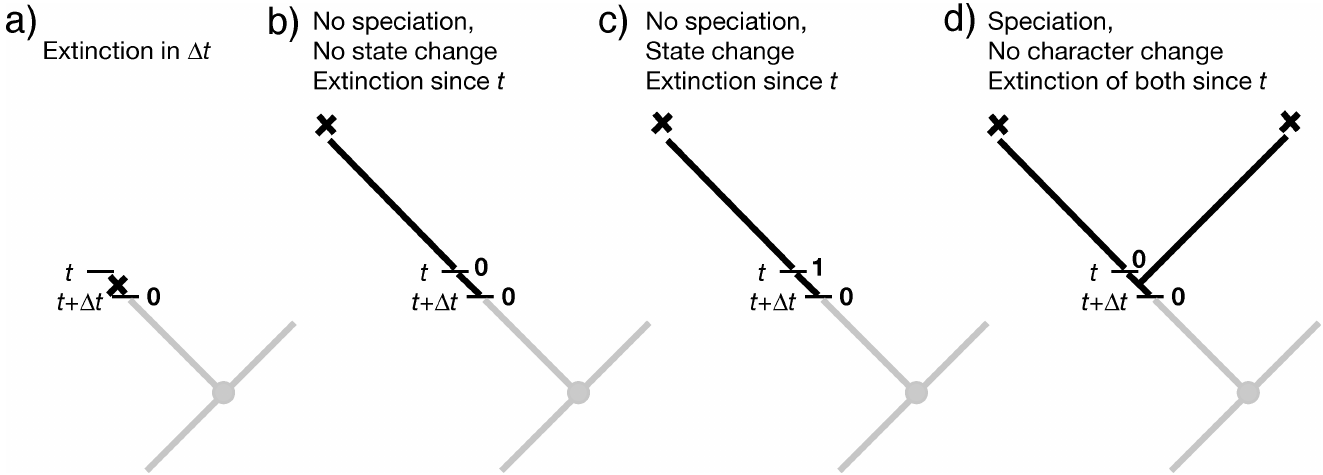
\includegraphics[width=0.9\textwidth]{\ResourcePath figures/BiSSE_Events_E.png}}
\caption{\small
    Possible events along a branch in the BiSSE model, used for deriving $E_0(t + \Delta t)$.
    This is Figure 3 in \citet{Maddison2007}.
}
\label{fig:BiSSE_Events_E}
\end{figure}

To convert these difference equations into differential equations, we again take the limit $\Delta t \rightarrow 0$:
\begin{equation}
    \frac{\mathrm{d}E_i(t)}{\mathrm{d}t} = \mu_i - \left(\lambda_i + \mu_i + q_{ij} \right)E_i(t) + q_{ij} E_j(t) + \lambda_i E_i(t)^2
    \label{eq:BiSSE_E}
\end{equation}

\subsubsection{Initial values: tips and sampling}
%%% TIPS %%%

The equations above describe how to get the answer at time $t + \Delta t$ assuming we already have the answer at time $t$.
How do we start this process?
The answer is with our character state observations, which are generally the tip state values.
If species $s$ has state $i$, then $D_{s,i}(0) = 1$ (probability is 1 at time 0 [the present] because we observed it for sure) and $E_i(0) = 0$ (probability 0 of being extinct at the present).
For all states other than $i$, $D_{s,j}(0) = 0$ and $E_j(0) = 1$.

We can adjust these initial conditions to allow for incomplete sampling.
If a proportion $\rho$ of species are included on the tree, we would instead set $D_{s,i}(0) = \rho$ (probability of having state $s$ \emph{and} of being on the tree) and $E_i(0) = 1-\rho$ (probability of absent, due to sampling rather than extinction).
This simple form of incomplete sampling assumes that any species is equally likely to be on the tree \citep{FitzJohn2009}.

\subsubsection{At nodes}
%%% NODE %%%

Equations (\ref{eq:BiSSE_D}) and (\ref{eq:BiSSE_E}) are the BiSSE ODEs, describing probabilities along the branches of a phylogeny.
We also need to specify what happens with the clade probabilities (the $D$s) at the nodes of the tree.
BiSSE assumes the ancestor (called $A$) and descendants (called $N$ and $M$) have the same state (\IE there is no cladogenetic character change).
The initial value for the ancestral branch going into a node (at time $t_A$) is then the product of the final values for each of the daughter branches coming out of that node, times the instantaneous speciation rate (to account for the observed speciation event):
\begin{equation}
    D_{A, i}(t_A) = D_{N, i}(t_A) D_{M, i}(t_A) \lambda_i
    \label{eq:BiSSE_node}
\end{equation}

\subsubsection{At the root}
%%% ROOT %%%

After we integrate Equations (\ref{eq:BiSSE_D}) and (\ref{eq:BiSSE_E}) from the tips to the root, dealing with nodes along the way via Equation~(\ref{eq:BiSSE_node}), we arrive at the root with the $D$ values (called $D_{R, i}$), one for each state.
These need to be combined somehow to get the overall likelihood of the data:
\begin{equation*}
    \text{Likelihood(tree, tip states)} = \sum_i D_{R, i} \, p_{R, i}
\end{equation*}
What probability weighting, $p_{R, i}$ should be used for the possible root states?
Sometimes a fixed approach is used, assuming that the prior root state probabilities are either all equal, or are the same as the observed tip state frequencies, or are the equilibrium state frequencies under the model parameters.
These assumptions do not have a real basis, however (unless there is some external data that supports them), and they can cause trouble \citep{Goldberg2008}.
An alternative is to use the BiSSE probabilities themselves to determine the root state weightings, essentially adjusting the weightings to be most consistent with the data and BiSSE parameters \citep{FitzJohn2009}.
Perhaps better is to treat the weightings as unknown parameters to be estimated.
These estimates are usually quite uncertain, but in a Bayesian framework, one can treat the $p_{R, i}$ as nuisance parameters and integrate over them. 

\begin{table}[h!]
	\centering
	\caption{\bf{\BiSSE model parameters and their interpretation}} \label{tab:Bparam}
	\begin{tabular}{ l l l }
		\toprule
		Parameter & Interpretation \\
		\midrule
		$\Psi$ & Phylogenetic tree with divergence times \\
		\rowcolor{gray!15} $T$ & Root age \\
		$q_{01}$ & Rate of transitions from 0 to 1 \\
		\rowcolor{gray!15} $q_{10}$ & Rate of transitions from 1 to 0 \\
		$\lambda_0$ & Speciation rate for state 0 \\
		\rowcolor{gray!15} $\mu_0$ & Extinction rate for state 0 \\
		$\lambda_1$ & Speciation rate for state 1 \\
		\rowcolor{gray!15} $\mu_1$ & Extinction rate for state 1 \\
	\end{tabular}
\end{table}

%%%%%%%%%%%%%%%%%%%%
%%%  MuSSE math  %%%
%%%%%%%%%%%%%%%%%%%%
\subsection{Equations for the multi-state birth-death process}

The entire derivation above can easily be expanded to accommodate an arbitrary number of states \citep{FitzJohn2012}.
The only extra piece is summing over all the possible state transitions.
%
% For $k$ states, we write a set of $k$ difference equations for $D_{N,0}(t+\Delta t), D_{N,1}(t+\Delta t), \ldots, D_{N,k}(t+\Delta t)$.
%\begin{align}
%		D_{N,i}(t + \Delta t) = & \;(1 - \mu_i\Delta t) \times \label{equation:DKStates} \\
%		& \;[  (1 - \sum\limits_{j \neq i}^k q_{ij}\Delta t)(1 - \lambda_i\Delta t)D_{N,i}(t) \nonumber\\
%		& \; + (1 - \lambda_i\Delta t)  \sum\limits_{j \neq i}^k q_{ij}\Delta t D_{N,j}(t) \nonumber\\
%		& \; + 2 (1 - \sum\limits_{j \neq i}^k q\Delta t) \lambda_i\Delta t E_i(t)D_{N,i}(t)] \nonumber
%\end{align}
%along with $E_0(t+\Delta t), E_1(t+\Delta t), \ldots, E_k(t+\Delta t)$:
%\begin{align}
%	E_i(t + \Delta t) = &\; \mu_i\Delta t +	\label{equation:ExtKStates}	\\
%				    	    & (1 - \mu_i\Delta t) \times \nonumber\\
%					    & \;[(1-\sum\limits_{j \neq i}^k q_{ij}\Delta t)(1-\lambda_i\Delta t)E_i(t) \nonumber\\
%					    & \;+ (1-\lambda_i\Delta t) \sum\limits_{j \neq i}^k q_{ij}\Delta t E_j(t) \nonumber\\
%					    & \;+ (1 - \sum\limits_{j \neq i}^k q\Delta t) \lambda_i\Delta t E_i(t)^2] \nonumber
%\end{align}
%
The resulting differential equations within the branches are:
\begin{align*}
    \frac{\mathrm{d}D_{N,i}(t)}{\mathrm{d}t} &= - \left(\lambda_i + \mu_i + \sum\limits_{j \neq i}^k q_{ij} \right)D_{N,i}(t) + \sum\limits_{j \neq i}^k q_{ij} D_{N,j}(t) + 2\lambda_iE_i(t)D_{N,i}(t) \\
    \frac{\mathrm{d}E_i(t)}{\mathrm{d}t} &= \mu_i - \left(\lambda_i + \mu_i + \sum\limits_{j \neq i}^k q_{ij} \right)E_i(t) + \sum\limits_{j \neq i}^k q_{ij} E_j(t) + \lambda_i E_i(t)^2
\end{align*}

%%%%%%%%%%%%%%%%%%%%%%
%%  Using RevBayes  %%
%%%%%%%%%%%%%%%%%%%%%%
\section{Using state-dependent diversification models with \RevBayes: the BiSSE model} \label{sec:CDBDP}

Now let's start to analyze an example in \RevBayes using the BiSSE model.
In \RevBayes, it's called ``CDBDP,'' meaning Character Dependent Birth Death Process.

\subsection{Read in the data}

Begin by reading in the observed tree and the character state data.
We have both stored in separate nexus files.
{\tt \begin{snugshade*}
\begin{lstlisting}
observed_phylogeny <- readTrees("data/primates_tree.nex")[1]
data <- readCharacterData("data/primates_activity_period.nex")
\end{lstlisting}
\end{snugshade*}}
Note, the character-dependent birth-death process currently uses always the first character/site in the alignment file.
We have therefore split the character dataset into several small files that include only one character each.

It will be convenient to pull out the list of tip names from the tree:
{\tt \begin{snugshade*}
\begin{lstlisting}
taxa <- observed_phylogeny.taxa()
\end{lstlisting}
\end{snugshade*}}

Our vectors of moves and monitors will be defined later, but here we initialize iterator variables for them:
{\tt \begin{snugshade*}
\begin{lstlisting}
mvi = 0
mni = 0
\end{lstlisting}
\end{snugshade*}}

Finally, we create a helper variable that specifies the number of states that the observed character has:
{\tt \begin{snugshade*}
\begin{lstlisting}
NUM_STATES = 2
\end{lstlisting}
\end{snugshade*}}
Using this variable we can easily change our script to use a different character with a different number of states,
essentially changing out model from BiSSE to MuSSE.
(This will also be handy in our later example with the hidden-state speciation and extinction model.)

\subsection{Specify the model}

The basic idea behind the model in this example is that speciation and extinction rates are dependent on a binary character, and the character transitions between its two possible states \citep{Maddison2007}.

\subsubsection{Priors on the rates}

We start by specifying prior distributions on the diversification rates.
We will assume here an identical prior distribution on each of the speciation and extinction rates.
Furthermore, we will use a normal distribution as the prior distribution on the log of each speciation and extinction rate.
Hence, we will use a mean of $\ln(\frac{\text{\#Taxa}}{2}) / \text{tree-age}$ which is the expected net diversification rate.
{\tt \begin{snugshade*}
\begin{lstlisting}
rate_mean <- ln( ln(367.0/2.0) / observed_phylogeny.rootAge() )
rate_sd <- 2.0
\end{lstlisting}
\end{snugshade*}}
Now we can specify our character-specific speciation and extinction rate parameters.
Because we will use the same prior for each rate, it's easy to specify them all in a \cl{for}-loop.
We set up moves at the same time; a sliding move is good for a log-transformed variable.
{\tt \begin{snugshade*}
\begin{lstlisting}
for (i in 1:NUM_STATES) {
    
     ### Create a lognormal distributed variable for the diversification rate
    log_speciation[i] ~ dnNormal(mean=rate_mean,sd=rate_sd) 
    speciation[i] := exp( log_speciation[i] )
    moves[++mvi] = mvSlide(log_speciation[i],delta=0.20,tune=true,weight=3.0)

    ### Create a lognormal distributed variable for the turnover rate
    log_extinction[i] ~ dnNormal(mean=rate_mean,sd=rate_sd) 
    extinction[i] := exp( log_extinction[i] )
    moves[++mvi] = mvSlide(log_extinction[i],delta=0.20,tune=true,weight=3.0)

}
\end{lstlisting}
\end{snugshade*}}

Next we specify the transition rates between the states 0 and 1, $q_{01}$ and $q_{10}$.
As a prior, we choose that each transition rate is drawn from an exponential distribution with a mean of 10 character state transitions over the entire tree. 
This is reasonable because we use this kind of model for traits that transition not-infrequently, and it leaves a fair bit of uncertainty.
(You may want to compare the posterior to the prior and/or check the resulting posterior estimates for different choices of the prior.)
{\tt \begin{snugshade*}
\begin{lstlisting}
rate_pr := observed_phylogeny.treeLength() / 10
rate_12 ~ dnExponential(rate_pr)
rate_21 ~ dnExponential(rate_pr)
\end{lstlisting}
\end{snugshade*}}
For both transition rate variables we specify a scaling move.
{\tt \begin{snugshade*}
\begin{lstlisting}
moves[++mvi] = mvScale( rate_12, weight=2 )
moves[++mvi] = mvScale( rate_21, weight=2 )
\end{lstlisting}
\end{snugshade*}}
Finally, we put the rates into a matrix, because this is what's needed by the function for the state-dependent birth-death process.
{\tt \begin{snugshade*}
\begin{lstlisting}
rate_matrix := fnFreeBinary( [rate_12, rate_21 ], rescaled=false)
\end{lstlisting}
\end{snugshade*}}
Note that we do not ``rescale'' the rate matrix.
Rate matrices for molecular evolution are rescaled to have an average rate of 1.0, but for this model we want estimates of the transition rates with the same time scale as the diversification rates.

\subsubsection{Prior on the root state}
Create a variable with the prior probabilities of each rate category at the root.
We are using a flat Dirichlet distribution as the prior on each state.
In this case we are actually estimating the prior frequencies of the root states.
There has been some discussion about this in \cite{FitzJohn2009}.
You could also fix the prior probabilities for the root states to be equal (generally not recommended), or use empirical state frequencies. 
{\tt \begin{snugshade*}
\begin{lstlisting}
rate_category_prior ~ dnDirichlet( rep(1,NUM_STATES) )
moves[++mvi] = mvDirichletSimplex(rate_category_prior,tune=true,weight=2)
\end{lstlisting}
\end{snugshade*}}

\subsubsection{Incomplete taxon sampling}

We know that we have sampled 233 out of 367 living primate species. 
To account for this we can set the sampling parameter as a constant node with a value of 233/367.
{\tt \begin{snugshade*}
\begin{lstlisting}
rho <- observed_phylogeny.ntips()/367
\end{lstlisting}
\end{snugshade*}}


\subsubsection{Root age}

The birth-death process requires a parameter for the root age.
In this exercise we use a fixed tree and thus we know the age of the tree.
{\tt \begin{snugshade*}
\begin{lstlisting}
root <- observed_phylogeny.rootAge()
\end{lstlisting}
\end{snugshade*}}

\subsubsection{The time tree}

Now we have all of the parameters we need to specify the full character state-dependent birth-death model.
We initialize the stochastic node representing the time tree.
{\tt \begin{snugshade*}
\begin{lstlisting}
timetree ~ dnCDBDP( rootAge           = root,
                    speciationRates   = speciation,
                    extinctionRates   = extinction, 
                    Q                 = rate_matrix,
                    pi                = rate_category_prior,
                    delta             = 1.0,
                    rho               = rho,
                    condition         = "survival",
                    taxa              = taxa )
\end{lstlisting}
\end{snugshade*}}
And then we attach data to it.
{\tt \begin{snugshade*}
\begin{lstlisting}
timetree.clamp( observed_phylogeny )
timetree.clampCharData( data )
\end{lstlisting}
\end{snugshade*}}

Finally, we create a workspace object of our whole model.
The \cl{model()} function traverses all of the connections and finds all of the nodes we specified.
{\tt \begin{snugshade*}
\begin{lstlisting}
mymodel = model(rate_matrix)
\end{lstlisting}
\end{snugshade*}}

\subsection{Running an MCMC analysis}

\subsubsection{Specifying monitors}

For our MCMC analysis, we set up a vector of \emph{monitors} to record the states of our Markov chain. 
The first monitor will model all numerical variables; we are particularly interesed in the rates of speciation, extinction, and transition.
{\tt \begin{snugshade*}
\begin{lstlisting}
monitors[++mni] = mnModel(filename="output/primates_BiSSE.log", printgen=1)
\end{lstlisting}
\end{snugshade*}}

The second monitor is a new type of monitor: an joint-ancestral-states monitor.
This monitor takes a draw from the joint posterior distribution of the ancestral states.
Thus, with this output file we will be able to make a nice plot with ancestral states.
{\tt \begin{snugshade*}
\begin{lstlisting}
monitors[++mni] = mnJointConditionalAncestralState(tree=timetree, cdbdp=timetree, type="Standard", printgen=1, withTips=true, withStartStates=false, filename="output/anc_states_primates_BiSSE.log")
\end{lstlisting}
\end{snugshade*}}
(Note that this is a bit different than the marginal ancestral state reconstructions commonly produced by, e.g., Mesquite or various R packages.
These joint draws are a self-consistent set of states across all nodes.
\citet{Pagel1999} discusses the differences.)

Finally, we add a screen monitor showing some updates during the MCMC run.
{\tt \begin{snugshade*}
\begin{lstlisting}
monitors[++mni] = mnScreen(printgen=10, rate_12, rate_21, speciation, extinction)
\end{lstlisting}
\end{snugshade*}}

\subsubsection{Initializing and running the MCMC simulation}

With a fully specified model, a set of monitors, and a set of moves, we can now set up the MCMC algorithm that will sample parameter values in proportion to their posterior probability. 
The \cl{mcmc()} function will create our MCMC object:
{\tt \begin{snugshade*}
\begin{lstlisting}
mymcmc = mcmc(mymodel, monitors, moves)
\end{lstlisting}
\end{snugshade*}}

First, we will run a pre-burnin to tune the moves and to obtain starting values from the posterior distribution.
{\tt \begin{snugshade*}
\begin{lstlisting}
mymcmc.burnin(generations=5000,tuningInterval=200)
\end{lstlisting}
\end{snugshade*}}

Now, run the MCMC:
{\tt \begin{snugshade*}
\begin{lstlisting}
mymcmc.run(generations=20000)
\end{lstlisting}
\end{snugshade*}}

\subsubsection{Summarizing ancestral states}

After our MCMC run has finished, we read-in again our samples from the joint-ancestral-state posterior distribution.
{\tt \begin{snugshade*}
\begin{lstlisting}
anc_states = readAncestralStateTrace("output/anc_states_primates_BiSSE.log")
\end{lstlisting}
\end{snugshade*}}
Then we can use this trace and our fixed tree to compute the posterior probabilities of the ancestral states and prepare the output for plotting.
We will use the function called \cl{ancestralStateTree} which stores the tree with ancestral states automatically in a file.
{\tt \begin{snugshade*}
\begin{lstlisting}
anc_tree = ancestralStateTree(tree=observed_phylogeny, ancestral_state_trace_vector=anc_states, include_start_states=false, file="output/anc_states_primates_BiSSE_results.tree", burnin=0, summary_statistic="MAP", site=0)
\end{lstlisting}
\end{snugshade*}}


\subsubsection{Plotting ancestral states}

Let us first plot the ancestral states mapped on the phylogeny.
We will use \R and the package \RevGadgets.
Execute the following code in \R.
\definecolor{shadecolor}{RGB}{200,200,200}
{\tt \begin{snugshade*}
\begin{lstlisting}
library(RevGadgets)

tree_file = "output/anc_states_primates_BiSSE_results.tree"

plot_ancestral_states(tree_file, summary_statistic="MAP",
                      tip_label_size=0,
                      xlim_visible=NULL,
                      node_label_size=0,
                      show_posterior_legend=TRUE,
                      node_size_range=c(2, 6),
                      alpha=0.75)

output_file = "RevBayes_Anc_States_BiSSE.pdf"
ggsave(output_file, width = 11, height = 9)
\end{lstlisting}
\end{snugshade*}}
\definecolor{shadecolor}{RGB}{183,207,237}
\begin{figure}[h!]
\centering
\fbox{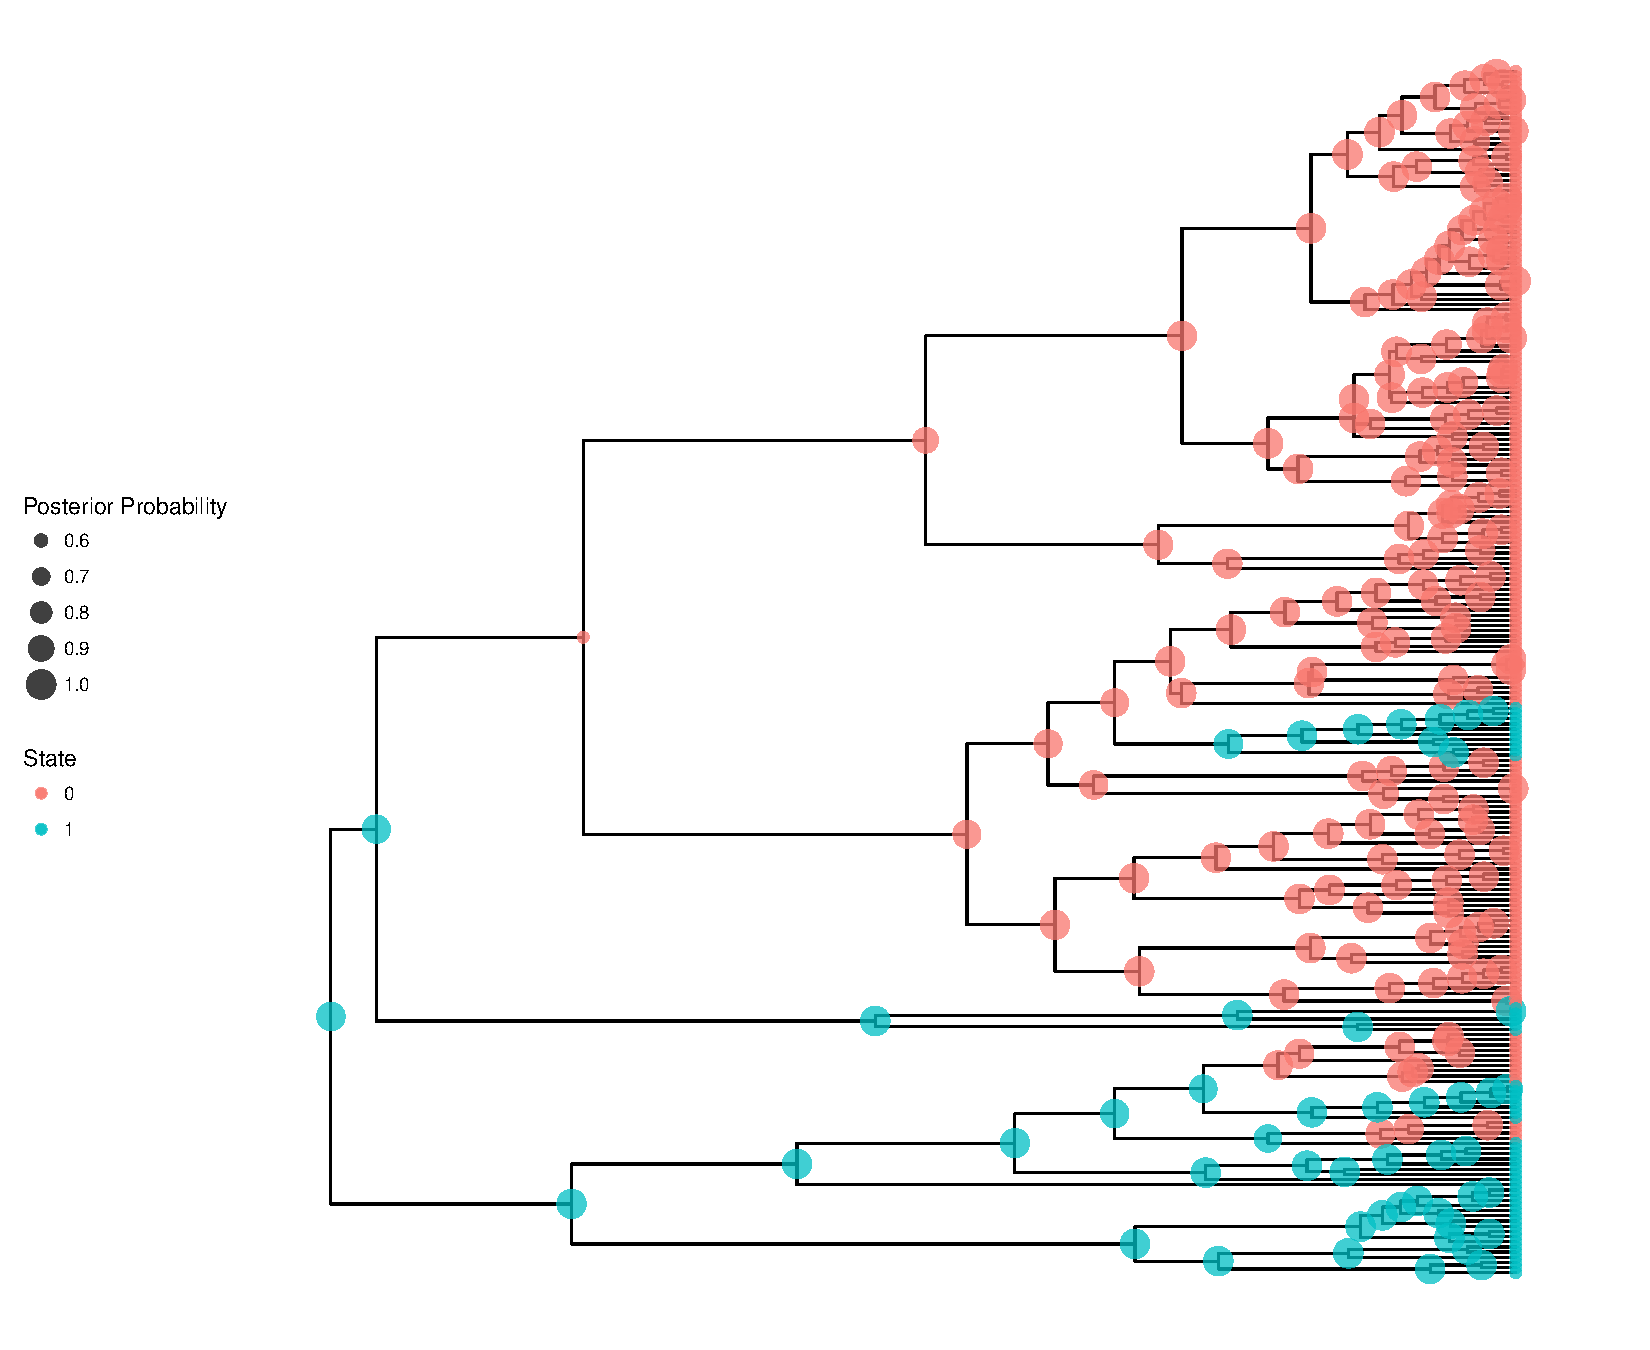
\includegraphics[width=\textwidth]{\ResourcePath figures/RevBayes_Anc_States_BiSSE.pdf}}
\caption{\small Estimated ancestral states for the activity period of primates.}
\label{fig:anc_states_BiSSE}
\end{figure}
The resulting plot is shown in Figure~\ref{fig:anc_states_BiSSE}.
We see both the maximum \emph{a posteriori} (MAP) estimate for each node as well as the posterior probability of the states represented by the size of the dots.

\subsubsection{Plotting diversification rates}

Now let us plot the diversification rate estimates.
Again, we are going to use \R for our plotting.
Specifically, we will use the package \texttt{ggplot2} but you can also use any other package that you prefer.
We are only taking advantage of reading in the tab-delimited file as a table and plot the different diversification rate parameters.
Note that we also rely on another provided \R script for plotting multiple plots in one file.
\definecolor{shadecolor}{RGB}{200,200,200}
{\tt \begin{snugshade*}
\begin{lstlisting}
library(ggplot2)
source("scripts/multiplot.R")

data <- read.table("output/primates_BiSSE.log",header=TRUE)

dat_ext  <- data.frame(dens = c(data$extinction.1, data$extinction.2), Type = rep(c("1", "2"), each = length(data$extinction.1)))
dat_spec <- data.frame(dens = c(data$speciation.1, data$speciation.2), Type = rep(c("1", "2"), each = length(data$extinction.1)))
dat_div  <- data.frame(dens = c(data$speciation.1-data$extinction.1, data$speciation.2-data$extinction.2), Type = rep(c("1", "2"), each = length(data$extinction.1)))
dat_rel  <- data.frame(dens = c(data$extinction.1/data$speciation.1, data$extinction.2/data$speciation.2), Type = rep(c("1", "2"), each = length(data$extinction.1)))

pdf("RevBayes_BiSSE_Results.pdf")

p1 <- ggplot(dat_spec, aes(x = dens, fill = Type)) + labs(title = "Speciation", x="Rate", y="Posterior Density") + geom_density(alpha = 0.5)
p2 <- ggplot(dat_ext, aes(x = dens, fill = Type)) + labs(title = "Extinction", x="Rate", y="Posterior Density") + geom_density(alpha = 0.5)
p3 <- ggplot(dat_div, aes(x = dens, fill = Type)) + labs(title = "Net-Diversification", x="Rate", y="Posterior Density") + geom_density(alpha = 0.5)
p4 <- ggplot(dat_rel, aes(x = dens, fill = Type)) + labs(title = "Relative Extinction", x="Rate", y="Posterior Density") + geom_density(alpha = 0.5)

multiplot(p1, p2, p3, p4)
dev.off()
\end{lstlisting}
\end{snugshade*}}
\begin{figure}[h!]
\centering
\fbox{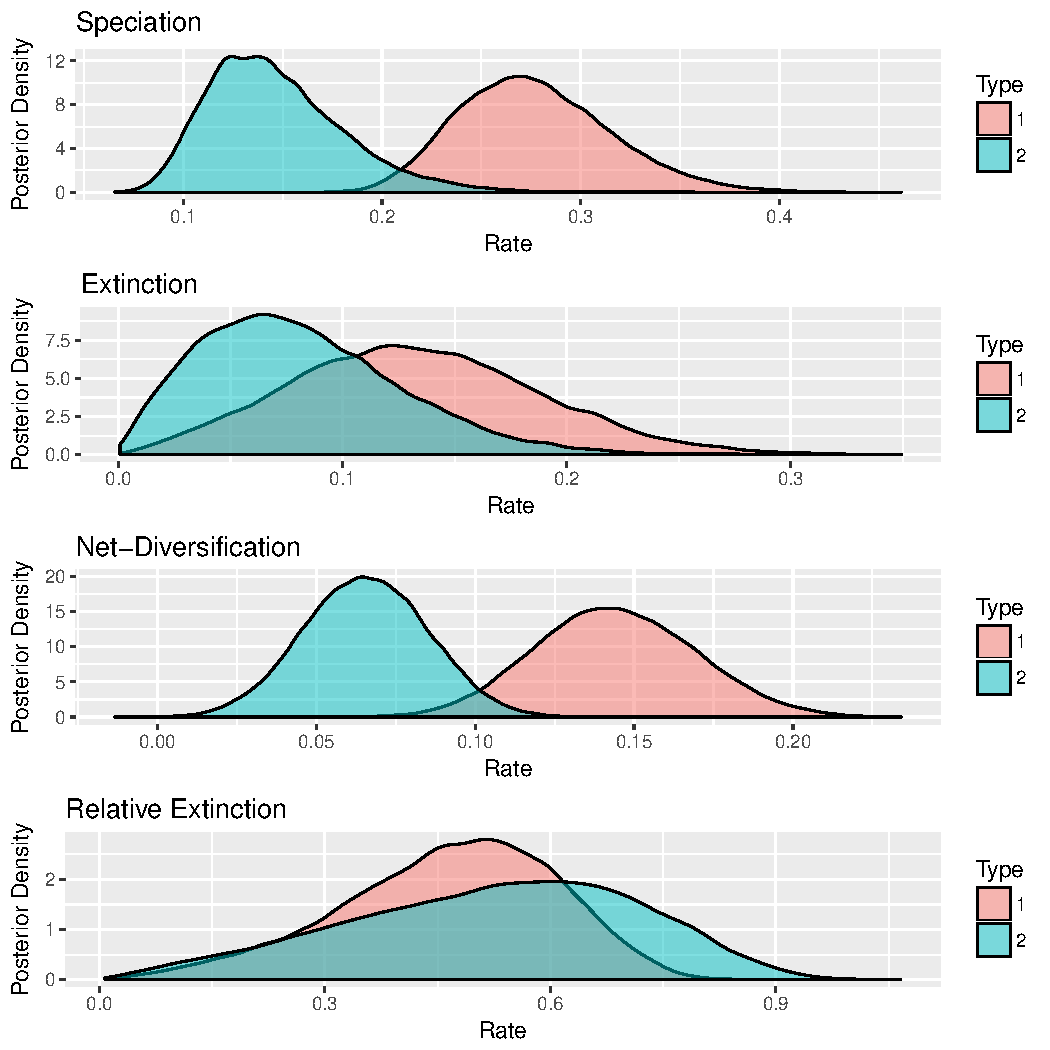
\includegraphics[width=\textwidth]{\ResourcePath figures/RevBayes_BiSSE_Results_activity_period.pdf}}
\caption{\small Estimated diversification rate for activity period (state 1 = Diurnal and state 2 = Nocturnal). We see that there is a noticeable difference in the estimated speciation rates but only little difference in the estimated extinction rates.}
\label{fig:div_rates_BiSSE}
\end{figure}


\definecolor{shadecolor}{RGB}{183,207,237}

%\impmark{The \Rev file for performing this analysis: \href{https://github.com/revbayes/revbayes_tutorial/raw/master/RB_DiversificationRateEpisodic_Tutorial/RevBayes_scripts/mcmc_EBD.Rev}{\cl{mcmc\_EBD.Rev}}.}
%\impmark{An \R file for plotting the output: \href{https://github.com/revbayes/revbayes_tutorial/raw/master/RB_DiversificationRateEpisodic_Tutorial/RevBayes_scripts/Plot_EBD_RevBayes.R}{\cl{Plot\_EBD\_RevBayes.R}}.}


\subsection{Exercise}

\begin{enumerate}
\item Run an MCMC simulation to estimate the posterior distribution of the speciation rate and extinction rate.
\item Visualize the state-specific diversification rates using \R.
\item Do you see evidence for rate differences between the two states?
\item Repeat this analysis for a different binary character.
\end{enumerate}


\bigskip
\section{Accommodating uncorrelated diversification rate changes: the HiSSE model}\label{sec:HiSSE_Theory}

BiSSE and MuSSE are powerful approaches for testing the association of a character
with diversification rate heterogeneity.
However, BiSSE has been shown to be prone to falsely identifying a positive association
when diversification rate shifts are correlated with a character \textit{not} included in the model \cite{Rabosky2015}.
One approach to reduce the possibility of falsely associating a character with diversification rate
heterogeneity is to incorporate a second, unobserved character into the model  \citep[i.e.\ a Hidden State-Dependent Speciation and Extinction (HiSSE) model;][]{Beaulieu2016}.
The changes in the unobserved character's state represent background diversification rate changes
that are not correlated with the oberved character.
See Figure \ref{fig:hisse} for a schematic overview of the HiSSE model, and Table \ref{tab:Hparam} for an explanation of the HiSSE model parameters.
Now let's set up and run a HiSSE analysis in \RevBayes.

\begin{figure}[h!]
\centering
\fbox{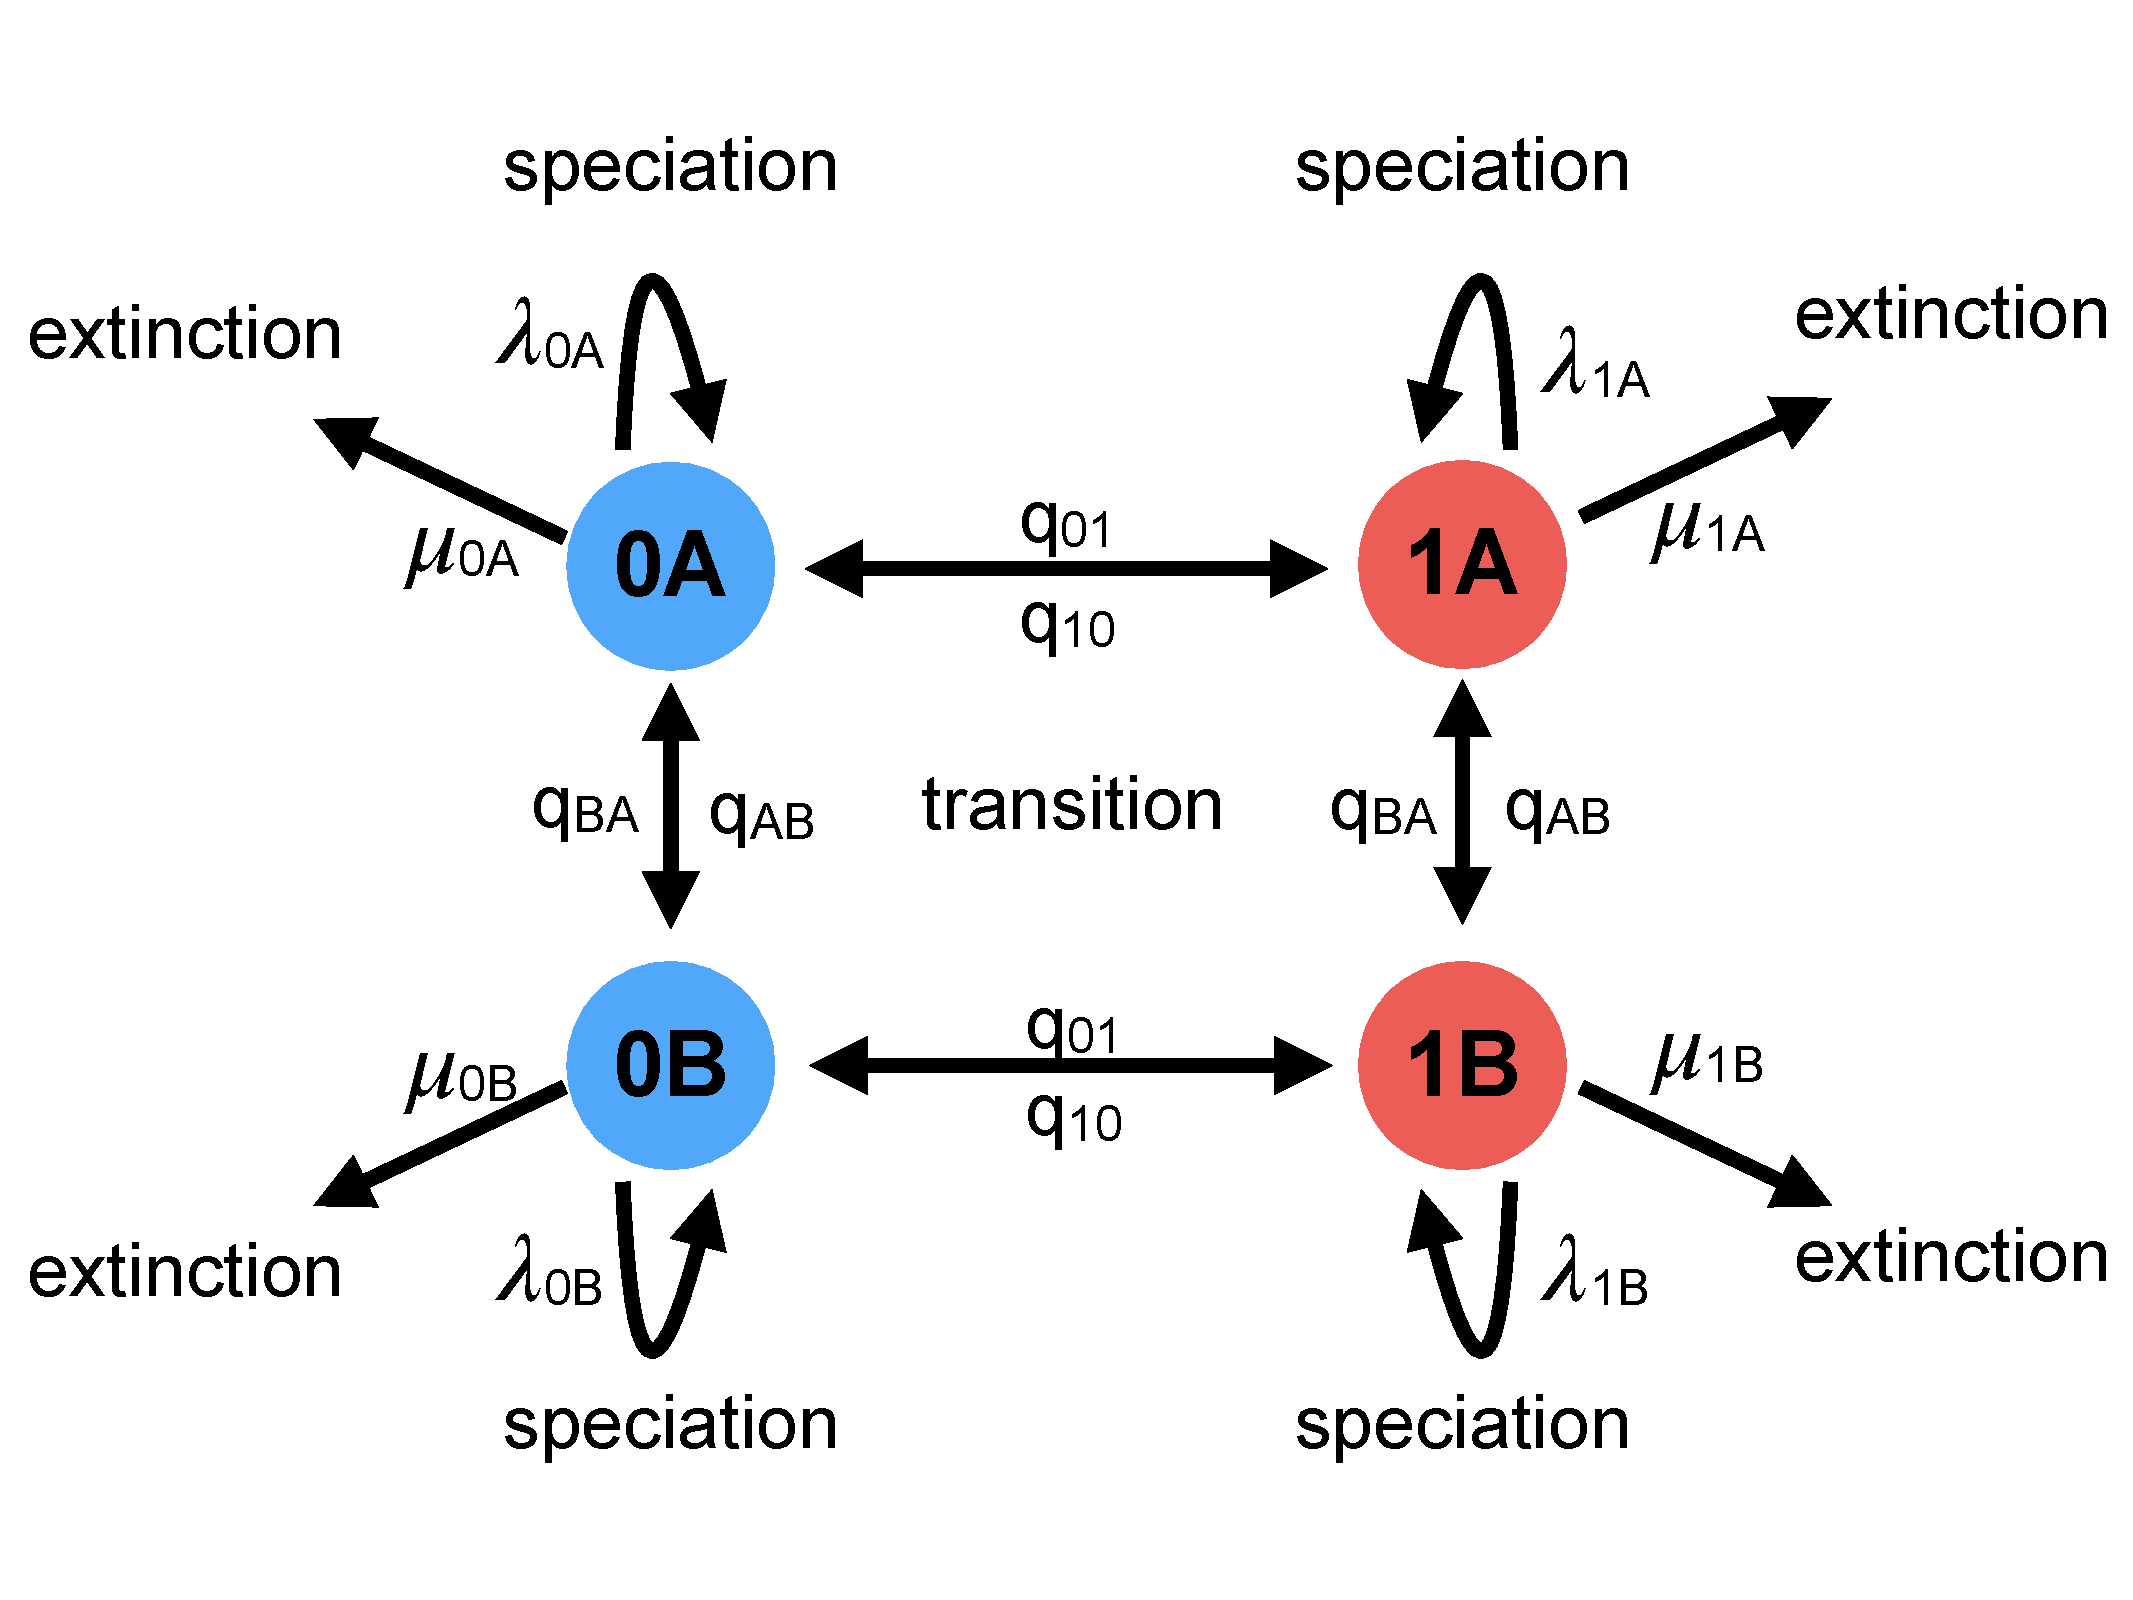
\includegraphics[width=\textwidth]{\ResourcePath figures/HiSSE.pdf}}
\caption{\small A schematic overview of the \HiSSE model. Each lineage has an observed binary state associated to it: state 0 (blue) or state 1 (red). 
Furthermore, there is a second, unobserved (hidden), binary character with states A or B.
The HiSSE model describes jointly the evolution of both of these two characters; a lineage
    must be in one of four different states: 0A, 0B, 1A, or 1B.
    We estimate separate speciation and extinction rates for each of these four states.
    Note that just like BiSSE can easily be extended to MuSSE,
    \RevBayes allows you to extend HiSSE models beyond binary observed and unobserved characters.}
\label{fig:HiSSE_Schematic}
\end{figure} \label{fig:hisse}



\begin{table}[t!]
	\centering
	\caption{\bf{\HiSSE model parameters and their interpretation}} \label{tab:Hparam}
	\begin{tabular}{ l l l }
		\toprule
		Parameter & Interpretation \\
		\midrule
		$\Psi$ & Phylogenetic tree with divergence times.\\
		\rowcolor{gray!15} $T$ & The root age.\\
		$q_{01}$ & The rate of shifts between observed states 0 to 1.\\
		\rowcolor{gray!15} $q_{10}$ & The rate of shifts between observed states 1 to 0.\\
		$q_{AB}$ & The rate of shifts between hidden states A to B.\\
		\rowcolor{gray!15} $q_{BA}$ & The rate of shifts between hidden states B to A.\\
        $\lambda_{0A}$ & Speciation rate for state 0A.\\
        \rowcolor{gray!15} $\mu_{0A}$ & Extinction rate for state 0A.\\
        $\lambda_{1A}$ & Speciation rate for state 1A.\\
        \rowcolor{gray!15} $\mu_{1A}$ & Extinction rate for state 1A.\\
        $\lambda_{0B}$ & Speciation rate for state 0B.\\
        \rowcolor{gray!15} $\mu_{0B}$ & Extinction rate for state 0B.\\
        $\lambda_{1B}$ & Speciation rate for state 1B.\\
        \rowcolor{gray!15} $\mu_{1B}$ & Extinction rate for state 1B.\\
	\end{tabular}
\end{table}


\subsection{Read the tree}

Begin by reading in the observed tree and the morphological data. 
We have both stored in separate nexus files.
{\tt \begin{snugshade*}
\begin{lstlisting}
observed_phylogeny <- readTrees("data/primates_tree.nex")[1]
data <- readCharacterData("data/primates_activity_period.nex")
\end{lstlisting}
\end{snugshade*}}
Note, the character-dependent birth-death process currently uses always the first character/site in the alignment file.
We have therefore split the morphological dataset into several small files that include only one morphological character each.

From the tree, we can get some helpful variables:
{\tt \begin{snugshade*}
\begin{lstlisting}
taxa <- observed_phylogeny.taxa()
\end{lstlisting}
\end{snugshade*}}

Additionally, we can initialize an iterator variable for our vector of moves and monitors:
{\tt \begin{snugshade*}
\begin{lstlisting}
mvi = 0
mni = 0
\end{lstlisting}
\end{snugshade*}}

Finally, we create a helper variable that specifies the number of states that the morphological character has.
{\tt \begin{snugshade*}
\begin{lstlisting}
NUM_STATES = 2
NUM_HIDDEN = 2
NUM_RATES = NUM_STATES * NUM_HIDDEN
\end{lstlisting}
\end{snugshade*}}
Using this variable we can easily change our script to use a different morphological character with a different number of states.
We will also use this variable in our second example on hidden-state speciation and extinction model. 


\subsubsection{Priors on rates}
We start by specifying prior distributions on the diversification rates.
We will assume here an identical prior distribution on the speciation and extinction rate.
Furthermore, we will use a normal distribution as the prior distribution on the log of the speciation and extinction rate.
Hence, we will use a mean of $\frac{\ln(\frac{\text{\#Taxa}}{2})}{\text{tree-age}}$ which is the expected net-diversification rate.
{\tt \begin{snugshade*}
\begin{lstlisting}
rate_mean <- ln( ln(367.0/2.0) / observed_phylogeny.rootAge() )
rate_sd <- 2.0
\end{lstlisting}
\end{snugshade*}}
Now we can specify our character-specific specification and extinction rate parameters.
As we just said before, we are going to use normal distributions for the prior on the log-speciation and log-extinction rate.
Here we will use a \cl{for}-loop to specify speciation and extinction parameters for each character, \EG two in a binary state case.
{\tt \begin{snugshade*}
\begin{lstlisting}
for (i in 1:NUM_STATES) {
    
     ### Create a lognormal distributed variable for the diversification rate
    log_speciation[i] ~ dnNormal(mean=rate_mean,sd=rate_sd) 
    speciation[i] := exp( log_speciation[i] )
    moves[++mvi] = mvSlide(log_speciation[i],delta=0.20,tune=true,weight=3.0)

    ### Create a lognormal distributed variable for the turnover rate
    log_extinction[i] ~ dnNormal(mean=rate_mean,sd=rate_sd) 
    extinction[i] := exp( log_extinction[i] )
    moves[++mvi] = mvSlide(log_extinction[i],delta=0.20,tune=true,weight=3.0)

}
\end{lstlisting}
\end{snugshade*}}
Now we need to create the variable for the hidden states.
{\tt \begin{snugshade*}
\begin{lstlisting}
for (i in 1:(NUM_HIDDEN-1)) {
    
    ### Create an exponential distributed variable for the diversification rate
    speciation_beta[i] ~ dnExp(1.0) 
    moves[++mvi] = mvScale(speciation_beta[i],lambda=0.20,tune=true,weight=2.0)        

    ### Create an normal distributed variable for the turnover rate
    extinction_beta[i] ~ dnNormal(0.0,1.0)
    moves[++mvi] = mvSlide(extinction_beta[i],delta=0.20,tune=true,weight=2.0)
    
}
\end{lstlisting}
\end{snugshade*}}
Finally, we match the rates to all possible ---hidden and observed--- states.
{\tt \begin{snugshade*}
\begin{lstlisting}
for (j in 1:NUM_HIDDEN) {
    for (i in 1:NUM_STATES) {
        if ( j == 1) {
            speciation[i] := exp( speciation_alpha[i] )
            extinction[i] := exp( extinction_alpha[i] )
        } else {
            index = i+(j*NUM_STATES)-NUM_STATES
            speciation[index] := speciation[index-NUM_STATES] * exp( speciation_beta[j-1] )
            extinction[index] := exp( extinction_alpha[i] + extinction_beta[j-1] )
        }
    }
}
\end{lstlisting}
\end{snugshade*}}
As before, we specify a rate prior.
{\tt \begin{snugshade*}
\begin{lstlisting}
rate_pr := observed_phylogeny.treeLength() / 10
rate_12 ~ dnExponential(rate_pr)
rate_21 ~ dnExponential(rate_pr)
\end{lstlisting}
\end{snugshade*}}
For both rate variable we specify a scaling move.
{\tt \begin{snugshade*}
\begin{lstlisting}
moves[++mvi] = mvScale( rate_12, weight=2 )
moves[++mvi] = mvScale( rate_21, weight=2 )
\end{lstlisting}
\end{snugshade*}}
Finally, we build a rate matrix for the relative-rate of change between categories.
This is because we need a rate matrix in our state-dependent birth-death process.
{\tt \begin{snugshade*}
\begin{lstlisting}
Q := [ rate_12, rate_21 ]
\end{lstlisting}
\end{snugshade*}}
Set up the transition rate matrix for hidden states.
We assume the transitions among the hidden states are all equal and drawn from an exponential distribution.
{\tt \begin{snugshade*}
\begin{lstlisting}
hidden_rate ~ dnExponential(rate_pr)
moves[++mvi] = mvScale(hidden_rate,lambda=0.2,tune=true,weight=5)

for (i in 1:(NUM_HIDDEN * (NUM_HIDDEN - 1))) {
    R[i] := hidden_rate
}
\end{lstlisting}
\end{snugshade*}}
Create the rate matrix for the combined observed and hidden states
{\tt \begin{snugshade*}
\begin{lstlisting}
rate_matrix := fnHiddenStateRateMatrix(Q, R, rescaled=false)
\end{lstlisting}
\end{snugshade*}}
A specific note here is that we do not rescale the rate matrix. 
This is very important because otherwise rate matrices, as used for molecular evolution, are always rescaled to have an average rate of 1.0.
If such a rescaled rate matrix was used, then you need to provide an overall rate scalar $\delta$.

\subsubsection{Prior on the root state}
Create a variable with the prior probabilities of each rate category at the root.
We are using a flat Dirichlet distribution as the prior on each state.
In this case we are actually estimating the prior frequencies of the root states.
There has been some discussion about this in \cite{FitzJohn2009}.
You could also fix the prior probabilities for the root states to be equal (generally not recommended), or use empirical state frequencies. 
{\tt \begin{snugshade*}
\begin{lstlisting}
rate_category_prior ~ dnDirichlet( rep(1,NUM_STATES) )
moves[++mvi] = mvDirichletSimplex(rate_category_prior,tune=true,weight=2)
\end{lstlisting}
\end{snugshade*}}

\subsubsection{Incomplete Taxon Sampling}

We know that we have sampled 233 out of 367 living primate species. 
To account for this we can set the sampling parameter as a constant node with a value of 233/367
{\tt \begin{snugshade*}
\begin{lstlisting}
rho <- observed_phylogeny.ntips()/367
\end{lstlisting}
\end{snugshade*}}


\subsubsection{Root age}

The birth-death process requires a parameter for the root age.
In this exercise we use a fix tree and thus we know the age of the tree.
Hence, we can get the value for the root from the \citet{MagnusonFord2012} tree.
{\tt \begin{snugshade*}
\begin{lstlisting}
root <- observed_phylogeny.rootAge()
\end{lstlisting}
\end{snugshade*}}

\subsubsection{The time tree}

Now we have all of the parameters we need to specify the full state-dependent birth-death model. 
We initialize the stochastic node representing the time tree.
{\tt \begin{snugshade*}
\begin{lstlisting}
timetree ~ dnCDBDP( rootAge           = root,
                    speciationRates   = speciation,
                    extinctionRates   = extinction, 
                    Q                 = rate_matrix,
                    pi                = rate_category_prior,
                    delta             = 1.0,
                    rho               = rho,
                    condition         = "survival",
                    taxa              = taxa )
\end{lstlisting}
\end{snugshade*}}
And then we attach data to it.
{\tt \begin{snugshade*}
\begin{lstlisting}
timetree.clamp( observed_phylogeny )
timetree.clampCharData( data )
\end{lstlisting}
\end{snugshade*}}

Finally, we create a workspace object of our whole model using the \cl{model()} function. 
{\tt \begin{snugshade*}
\begin{lstlisting}
mymodel = model(rate_matrix)
\end{lstlisting}
\end{snugshade*}}

The \cl{model()} function traversed all of the connections and found all of the nodes we specified. 


\subsection{Running an MCMC analysis}

\subsubsection{Specifying Monitors}

For our MCMC analysis, we set up a vector of \emph{monitors} to record the states of our Markov chain. 
For more details 
{\tt \begin{snugshade*}
\begin{lstlisting}
monitors[++mni] = mnModel(filename="output/primates_HiSSE.log", printgen=1)
monitors[++mni] = mnJointConditionalAncestralState(tree=timetree, cdbdp=timetree, type="NaturalNumbers", printgen=1, withTips=true, withStartStates=false, filename="output/anc_states_primates_HiSSE.log")
monitors[++mni] = mnScreen(printgen=100, Q, R)
\end{lstlisting}
\end{snugshade*}}

\subsubsection{Initializing and Running the MCMC Simulation}

With a fully specified model, a set of monitors, and a set of moves, we can now set up the MCMC algorithm that will sample parameter values in proportion to their posterior probability. 
The \cl{mcmc()} function will create our MCMC object:
{\tt \begin{snugshade*}
\begin{lstlisting}
mymcmc = mcmc(mymodel, monitors, moves)
\end{lstlisting}
\end{snugshade*}}

First, we will run a pre-burnin to tune the moves and to obtain starting values from the posterior distribution.
{\tt \begin{snugshade*}
\begin{lstlisting}
mymcmc.burnin(generations=5000,tuningInterval=200)
\end{lstlisting}
\end{snugshade*}}

Now, run the MCMC:
{\tt \begin{snugshade*}
\begin{lstlisting}
mymcmc.run(generations=20000)
\end{lstlisting}
\end{snugshade*}}


\subsubsection{Summarizing ancestral states}
After the MCMC run we summarize and estimate the joint-ancestral-state estimates.
{\tt \begin{snugshade*}
\begin{lstlisting}
anc_states = readAncestralStateTrace("output/anc_states_primates_HiSSE.log")
anc_tree = ancestralStateTree(tree=observed_phylogeny, ancestral_state_trace_vector=anc_states, include_start_states=false, file="output/anc_states_primates_HiSSE_results.tree", burnin=0, summary_statistic="MAP", site=0)
\end{lstlisting}
\end{snugshade*}}



\subsubsection{Plotting diversification rates}
Again, we plot the diversification rate as before.
\definecolor{shadecolor}{RGB}{200,200,200}
{\tt \begin{snugshade*}
\begin{lstlisting}
library(ggplot2)
source("scripts/multiplot.R")

data <- read.table("output/primates_HiSSE.log",header=TRUE)

start <- round(0.5*length(data$extinction.1))
end   <- length(data$extinction.1)

HiSSE_types <- rep(c("1A", "2A", "1B", "2B"), each = length(data$extinction.1[start:end]))
dat_ext  <- data.frame(dens = c(data$extinction.1[start:end], data$extinction.2[start:end], data$extinction.3[start:end], data$extinction.4[start:end]), Type = HiSSE_types)
dat_spec <- data.frame(dens = c(data$speciation.1[start:end], data$speciation.2[start:end], data$speciation.3[start:end], data$speciation.4[start:end]), Type = HiSSE_types)
dat_div  <- data.frame(dens = c(data$speciation.1[start:end]-data$extinction.1[start:end], data$speciation.2[start:end]-data$extinction.2[start:end], data$speciation.3[start:end]-data$extinction.3[start:end], data$speciation.4[start:end]-data$extinction.4[start:end]), Type = HiSSE_types)
dat_rel  <- data.frame(dens = c(data$extinction.1[start:end]/data$speciation.1[start:end], data$extinction.2[start:end]/data$speciation.2[start:end], data$extinction.3[start:end]/data$speciation.3[start:end], data$extinction.4[start:end]/data$speciation.4[start:end]), Type = HiSSE_types)


pdf("RevBayes_HiSSE_Results.pdf")

p1 <- ggplot(dat_spec, aes(x = dens, fill = Type)) + labs(title = "Speciation", x="Rate", y="Posterior Density") + geom_density(alpha = 0.5) + guides(fill=guide_legend(ncol=2,byrow=TRUE))
p2 <- ggplot(dat_ext, aes(x = dens, fill = Type)) + labs(title = "Extinction", x="Rate", y="Posterior Density") + geom_density(alpha = 0.5) + guides(fill=guide_legend(ncol=2,byrow=TRUE))
p3 <- ggplot(dat_div, aes(x = dens, fill = Type)) + labs(title = "Net-Diversification", x="Rate", y="Posterior Density") + geom_density(alpha = 0.5) + guides(fill=guide_legend(ncol=2,byrow=TRUE))
p4 <- ggplot(dat_rel, aes(x = dens, fill = Type)) + labs(title = "Relative Extinction", x="Rate", y="Posterior Density") + geom_density(alpha = 0.5) + guides(fill=guide_legend(ncol=2,byrow=TRUE))

multiplot(p1, p2, p3, p4)
dev.off()

$
\end{lstlisting}
\end{snugshade*}}
\begin{figure}[h!]
\centering
\fbox{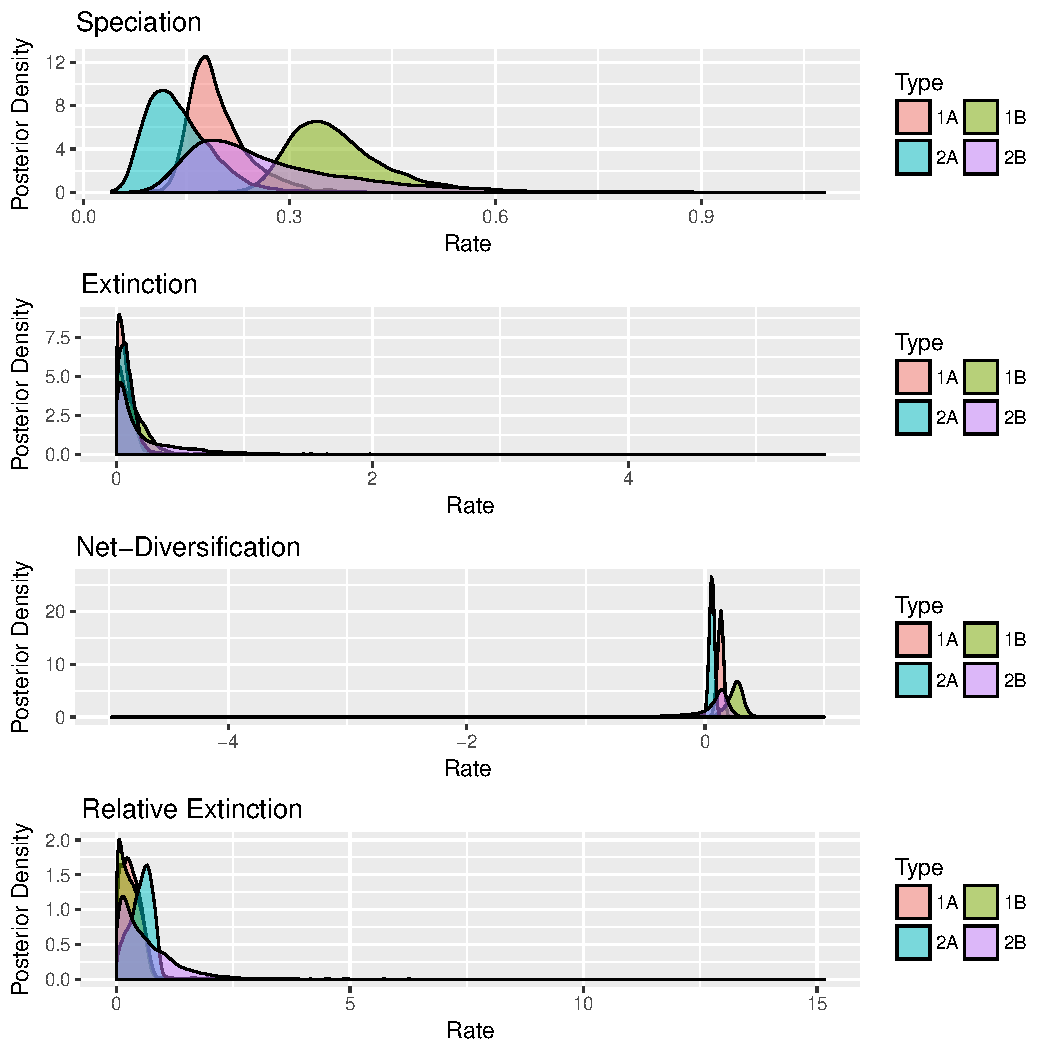
\includegraphics[width=\textwidth]{\ResourcePath figures/RevBayes_HiSSE_Results.pdf}}
\caption{\small Estimated diversification rate for activity period (state 1 = Diurnal and state 2 = Nocturnal).}
\label{fig:div_rates_HiSSE}
\end{figure}


\definecolor{shadecolor}{RGB}{183,207,237}

%\impmark{The \Rev file for performing this analysis: \href{https://github.com/revbayes/revbayes_tutorial/raw/master/RB_DiversificationRateEpisodic_Tutorial/RevBayes_scripts/mcmc_EBD.Rev}{\cl{mcmc\_EBD.Rev}}.}
%\impmark{An \R file for plotting the output: \href{https://github.com/revbayes/revbayes_tutorial/raw/master/RB_DiversificationRateEpisodic_Tutorial/RevBayes_scripts/Plot_EBD_RevBayes.R}{\cl{Plot\_EBD\_RevBayes.R}}.}


\subsection{Exercise}

\begin{enumerate}
\item Run an MCMC simulation to estimate the posterior distribution of the speciation rate and extinction rate.
\item Visualize the state-specific diversification rates using \R.
\item Do you see evidence for rate differences between the two states?
\item Do you see differences to the previous \BiSSE estimates?
\item Repeat this analysis for a different binary morphological character.
\end{enumerate}



\bigskip
\section{Accommodating both cladogenetic and anagenetic changes: the ClaSSE model}\label{sec:ClaSSE}

In the previous examples we have modeled all character state transitions
as anagenetic changes.
Anagenetic changes occur along the branches of a phylogeny, within a lineage.
Cladogenetic changes, on the other hand, occur only at speciation events.
They represent changes in a character state that may be associated with speciation events
due to increased reproductive isolation,
for example colonizing a new geographic area or a shift in chromosome number.

A major challenge for all phylogenetic models of cladogenetic character change
is accounting
for unobserved speciation events due to lineages going extinct
and not leaving any extant descendants \citep{Bokma2002},
or due to incomplete sampling of lineages in the present.
Teasing apart
the phylogenetic signal for cladogenetic and anagenetic processes given
unobserved speciation events is a major difficulty.
Commonly used biographic models like the
dispersal-extinction-cladogenesis \citep[DEC;][]{Ree2008} simply ignore
unobserved speciation events and so result in biased
estimates of cladogenetic versus anagenetic change.

This bias can be avoided by using the 
Cladogenetic State change Speciation and Extinction
(ClaSSE) model \citep{Goldberg2012},
which accounts for unobserved speciation events
by jointly modeling both character evolution
and the phylogenetic birth-death process.
ClaSSE models extend other SSE models by incorporating both cladogenetic 
and anagenetic character evolution.
This approach has been used to model biogeographic range evolution \citep{Goldberg2011}
and chromosome number evolution \citep{Freyman2017}.

Here we will use \RevBayes to examine biogeographic range evolution in the primates.
We will model biogeographic range evolution similar to a DEC model, 
however we will use ClaSSE at to account for speciation events unobserved due 
to extinction or incomplete sampling.


\bibliographystyle{sysbio}
\bibliography{\GlobalResourcePath refs}


Version dated: \today


\end{document}
